\documentclass[a4paper,11pt,oneside]{book}

\linespread{1.25}

\usepackage[utf8]{inputenc}

\usepackage{amsmath,amsfonts,amsthm,amssymb,dsfont}
\usepackage{graphicx,wrapfig,lipsum}
\usepackage[section]{placeins}
\usepackage{comment}\usepackage{float}
\usepackage{qcircuit}
\usepackage{tikz}


\usepackage[numbers,sort&compress]{natbib}

\usepackage{tikz}
\usetikzlibrary{shapes.geometric,decorations.markings}
\usepackage{subfigure}

\usepackage{slashed}

\usepackage[english]{babel}

\usepackage{listings}
\usepackage{xcolor}

\lstset{
  language=Python,
  basicstyle=\ttfamily\small,
  commentstyle=\color{gray},
  stringstyle=\color{gray},
  showstringspaces=false,
  breaklines=true,
  frame=single,
  columns=flexible,
}



\hyphenpenalty=10000
\exhyphenpenalty=10000
\sloppy


%---------------------------------------------------------------
%   PAGE  STYLE
%---------------------------------------------------------------

\voffset -1in
\hoffset -1in

\setlength{\marginparsep}{0mm}
\setlength{\parskip}{2mm}
\setlength{\textheight}{22.7cm}
\textwidth  .72\paperwidth
\addtolength\textheight{\topskip}


\topmargin   .05\paperheight
\headheight  .02\paperheight
\headsep     .03\paperheight
\footskip    .07\paperheight
\oddsidemargin .14\paperwidth
\evensidemargin .14\paperwidth
\marginparwidth .11\paperwidth



%-------------------------------------------------------------
%   DOCUMENT
%-------------------------------------------------------------

\begin{document}

%-------------------------------------------------------------
%	TITLE PAGE
%-------------------------------------------------------------

\begin{titlepage}
\begin{center}



\includegraphics[scale=0.35]{logo} \vspace{0.5cm}

\textsc{\Large Undergraduate Dissertation Report } \vspace{0.5cm} % Thesis type


\rule{14cm}{0.05cm} \vspace{0.4cm} % Horizontal line


\Large{\textbf{   The Mathematics of \\ Quantum Theory \& Computing  }}\vspace{0.4cm} % Thesis title

\rule{14cm}{0.05cm} \vspace{1.5cm} % Horizontal line
 
\large{\textit{by:}} \\
\Large{Dexter O'Neill}  %AUTHOR

\vspace{2cm}

\large \textit{
A report submitted in fulfillment of the requirements\\ 
for the BSc Hons - Mathematics and Computer Science} 

\vspace{0.3cm} % University requirement text

\textit{of the}

\vspace{0.4cm}

School of Mathematics and Computer Science,\\
Department of Mathematics,\\ 
Faculty of Science and Engineering,\\ 
Swansea University

\vspace{1.0cm} 

\today
 

\end{center}
\end{titlepage}


%--------------------------------------------------------------------
%	ABSTRACT PAGE
%--------------------------------------------------------------------
\newpage 
\pagenumbering{roman}
\setcounter{page}{2}


\addcontentsline{toc}{chapter}{Abstract}

\chapter*{Abstract}

This report introduces the mathematical foundations of quantum theory and computing. Starting with developing key concepts including linear algebra, probability, Hilbert spaces, Dirac notation, and linear operators. Building on these concepts, the report then develops the mathematical framework for quantum phenomena including superposition, interference, uncertainty, measurement, and entanglement. The report then transitions to contextualising this framework within computation. Qubits, quantum gates and circuits, algorithms, and accessible quantum programming tools are all described starting from their mathematical basis. This report bridges theory to practice, providing an introduction to quantum theory and its computational potential.



%-----------------------------------------------------------------
%	LIST OF CONTENTS/FIGURES/TABLES PAGES
%-----------------------------------------------------------------

\newpage

\addcontentsline{toc}{chapter}{Table of Contents}

\tableofcontents 

%--------------------------------------------------------------------
%	INTRODUCTION
%--------------------------------------------------------------------

\newpage

\pagenumbering{arabic}

\chapter{Introduction}


\begin{quote}
\textit{"Nature isn't classical, dammit, and if you want to make a simulation of nature, you'd better make it quantum mechanical"}  \\
\hfill -- Richard Feynman
\end{quote}


\noindent Quantum computing represents the pinnacle of modern computation power and is the future of the field. As the scalability of quantum computing advances, we will see a shift in all technological infrastructures, with everyone trying to keep up with the tremendous leap in computing capabilities. Quantum computing harnesses the phenomena/principles of quantum mechanics, including; Superposition, Interference, and Entanglement, to create a new non-classical computer. Quantum computers hold the potential to solve problems previously thought to be unsolvable by classical computers. Proof of this potential was demonstrated when Google claimed quantum supremacy in 2019. In [1], quantum supremacy was described as "the era of quantum supremacy, when we will be able to perform tasks with controlled quantum systems going beyond what can be achieved with ordinary digital computers." in other words, quantum supremacy is the point in time when the computational abilities of a quantum computer surpass that of a classical computer. Google's claim of quantum supremacy was by their quantum processor 'Sycamore'. As detailed in [2], the feat was a computational problem, it was estimated it would have taken one of the world's fastest classical supercomputers 'Summit' 10,000 years to complete, and Sycamore finished it in 200 seconds. The proficiency of these machines is likely to revolutionize industries such as cryptography and cyber security, materials science, AI, optimization, and the pharmaceutical research industry. One point to note about this achievement of Google is that the problem was a program completing a hyper specific task that takes advantage of the alternative underpinning logic quantum computers use. Therefore it is often sensationalised, so we must remember to take into account that while this is a first step it is a long way off a general out performance of classical computers. To paraphrase [4], the biggest opposition to Google's claim of quantum supremacy came from IBM who disputed that the task would take at best 10,000 years on a classical machine. They claimed the same task can be simulated on a classical computer with an upper bound of 2.5 days. IBM also stated that the threshold of the original meaning of the term proposed by John Preskill had not been met.

\noindent To investigate the extent of the prospect of quantum computing this dissertation examines the concepts of quantum theory that make up quantum computing then going into quantum computing. The goal will be to develop an understanding of some key topics such as; quantum theory phenomena, quantum computing logic and circuits, and quantum algorithms and their impact. Another goal is to demonstrate a quantum program using quantum programming tools like Qiskit. These aims will also help us fully realise the potential of quantum computing.

\noindent We begin with the mathematics of quantum theory, this section will give a detailed description on the principles of quantum mechanics that underpin quantum computers and their physical implementation. This will develop a solid background for understanding the later topics. Following this we delve into quantum logic and algorithms, explaining how qubits differ from bits, leading into the difference between classical and quantum mechanical computing logic (quantum gates). We will study some quantum computing algorithms, for example, explaining how Grover's search algorithm operates. To finish that section tools for programming on quantum computers and simulation will be discussed, with example usage of Qiskit. This will be followed by a conclusion where we will reflect on the impact quantum computers could have on areas, including; quantum simulations, the philosophical implications of AI on quantum computers, and quantum cryptography. Challenges of quantum computing and the structure of qubits and quantum computers will also be touched on and sources to delve into these topics in detail will be provided. 



%--------------------------------------------------------------------
%	THEMED CHAPTERS
%--------------------------------------------------------------------


\newpage

\chapter{Mathematics of Quantum Theory}

\section{Introduction}

\noindent These foundations of quantum theory aim to give a surface-level understanding in order to describe how it is leveraged to create quantum computer systems capable of outperforming classical systems. The section will begin with the mathematical necessities, and then move onto applying these tools to understand and mathematically represent quantum phenomena. Quantum mechanics is deeply intertwined with quantum computing, it is a branch of physics that aims to understand matter and energy on a very small, atomic, and sub-atomic scale. Unlike classical physics where everything acts in a deterministic manner, in quantum mechanics the world operates on a probabilistic framework. Particles are described as clouds of probabilities rather than solid ball-like particles. A law that demonstrates this indeterministic world well is Heisenberg's Uncertainty Principle, here $\Delta x$ is the uncertainty in position, $\Delta p$ is the uncertainty in momentum and $\hbar$ is the reduced Planck constant, defined as $\hbar = \frac{h}{2\pi}$ from [5]:

\[
\Delta x \cdot \Delta p \geq \frac{\hbar}{2}
\]

\noindent To paraphrase Dirac [3], Heisenberg's Uncertainty Principle shows the fundamental limitations of simultaneous measurement of two values, as long as they don't commute (the measurement of one property influences the other property). Essentially when measuring a pair of properties that conform to this principle (e.g. position and momentum), the act of measuring the value of one property more accurately, leads to the accuracy that the second property can be measured at, to decrease. This topic will be analysed in further detail later this chapter. Additional key concepts we will look to understand in this section are Superposition, Quantum Entanglement and Quantum teleportation.
\\
First, we will set the stage for understanding how quantum mechanics drives the development of quantum computers and will prepare the reader with the preliminaries needed for fully understanding the subsequent sections.



\section{Mathematical Basis/Preliminaries}

\subsection{Linear Algebra}

Linear Algebra is a crucial area of mathematics necessary for the mathematical formulation and providing a framework for understanding quantum theory. Here we will cover the essential linear algebra tools. Concepts like quantum states, qubits and quantum gates can be naturally described using some of these tools such as, vector spaces, matrices and linear transformations. For reference, definitions of fields and vector spaces can be found in appendix A.



\subsubsection{Inner Product Spaces}

An \textbf{inner product space} is a vector space \( V \) over a field \( \mathbb{F} \), equipped with an \textbf{inner product}:
\[
\langle \mathbf{u}, \mathbf{v} \rangle: V \times V \to \mathbb{F}
\]
Satisfying these properties, for all \( \mathbf{u}, \mathbf{v}, \mathbf{w} \in V \) and scalars \( a \in \mathbb{F} \):
\begin{enumerate}
    \item \textbf{Conjugate Symmetry}: \( \langle \mathbf{u}, \mathbf{v} \rangle = \overline{\langle \mathbf{v}, \mathbf{u} \rangle} \).
    \item \textbf{Linearity in the First Argument}: \( \langle a\mathbf{u} + \mathbf{v}, \mathbf{w} \rangle = a \langle \mathbf{u}, \mathbf{w} \rangle + \langle \mathbf{v}, \mathbf{w} \rangle \).
    \item \textbf{Positivity}: \( \langle \mathbf{v}, \mathbf{v} \rangle \geq 0 \), \(\forall \mathbf{v} \in V\)
 with equality if and only if \( \mathbf{v} = \mathbf{0} \).
\end{enumerate}


\noindent A common example is \( \mathbb{C}^n \) with the \textbf{inner product}:
\begin{equation}
\langle \mathbf{u}, \mathbf{v} \rangle = \sum_{i=1}^{n} u_i \overline{v_i}.
\end{equation}

\subsubsection{Orthogonality}

Two vectors \( \mathbf{u}, \mathbf{v} \in V \) are said to be \textbf{orthogonal} if their inner product is zero:
\[
\langle \mathbf{u}, \mathbf{v} \rangle = 0.
\]



\subsubsection{Normalization}
A vector \( \mathbf{v} \in V \) is \textbf{normalized} if its norm is 1, where the norm is defined as:
\begin{equation}
\|\mathbf{v}\| = \sqrt{\langle \mathbf{v}, \mathbf{v} \rangle}.
\end{equation}

\noindent In quantum mechanics, quantum state vectors must be normalized to satisfy probability conservation.

\subsubsection{Orthonormality}
A set of vectors \( \{\mathbf{v}_1, \mathbf{v}_2, \dots, \mathbf{v}_n\} \) is \textbf{orthonormal} if:
\begin{enumerate}
    \item The vectors are all \textbf{orthogonal} with every other vector: \( \langle \mathbf{v}_i, \mathbf{v}_j \rangle = 0 \) for \( i \neq j \).
    \item Each vector is \textbf{normalized}: \( \langle \mathbf{v}_i, \mathbf{v}_i \rangle = 1 \).
\end{enumerate}


\subsubsection{Basis of a Vector Space}
A set of vectors \( \{\mathbf{v}_1, \mathbf{v}_2, \dots, \mathbf{v}_n\} \) in \( V \) is a \textbf{basis} of the vector space if:
\begin{enumerate}
    \item It is \textbf{linearly independent}, so no vector in the set can be written as a linear combination of the others.
    \item It \textbf{spans} \( V \), so every \( \mathbf{v} \in V \) can be written as a linear combination of the basis vectors:
    \[
    \mathbf{v} = a_1 \mathbf{v}_1 + a_2 \mathbf{v}_2 + \dots + a_n \mathbf{v}_n, \quad a_i \in \mathbb{F}.
    \]
\end{enumerate}

\noindent If a basis consists of \( n \) vectors, the vector space has \textbf{dimension} \( n \), written as \( \dim V = n \).  \\
\noindent From inner product spaces to here reference [8] was used. 

\subsubsection{Eigenvectors and Eigenvalues}
Let \( A \) be a square matrix. A vector \( \mathbf{v} \) is an \textbf{eigenvector} of \( A \) if:
\begin{equation}
    A\mathbf{v} = \lambda \mathbf{v},
\end{equation}
\noindent where \( \lambda  \) is a scalar element of \( \mathbb{F} \) and the corresponding \textbf{eigenvalue} to the eigenvector. The eigenvalues are found by solving the characteristic polynomial:
\begin{equation}
    \det(A - \lambda I) = 0,
\end{equation}
where \( I \) is the identity matrix. The set of all eigenvalues is called the \textbf{spectrum} of \( A \).\\

\noindent \textbf{Note} you can see by equation 2.3 that multiplying the eigenvector \( \mathbf{v} \) by \( A \) does not affect the direction of the vector it just scales it by the scalar \( \lambda  \). In quantum mechanics properties such as energy or momentum are represented by hermitian operators. The eigenvalues represent potential measurement results, and the eigenvectors represent the potential states the system could collapse to upon measurement. [7] \& [9]


\subsubsection{Hermitian Matrices}

A \textbf{Hermitian matrix} is a square matrix with complex entries that is equal to its own conjugate transpose. That is, for a Hermitian matrix \( A \), we have:
\begin{equation}
A = A^\dagger,
\end{equation}
where \( A^\dagger \) denotes the conjugate transpose of \( A \). [10]
\\

\noindent \textbf{Note:} Hermitian matrices have two important properties:
\begin{enumerate}
    \item All eigenvalues of a Hermitian matrix are real.
    \item Eigenvectors corresponding to distinct eigenvalues are orthogonal.
\end{enumerate}

\noindent These properties make it clear as to why Hermitian matrices particularly useful for representing observables. Since eigenvalues correspond to possible measurement outcomes, Hermitian operators ensure that these outcomes are real. [9]


\subsubsection{Unitary Matrices}
A \textbf{Unitary matrix} satisfies the following equation:
\begin{equation}
U^\dagger U = UU^\dagger = I
\end{equation}
So can see that $U^\dagger$ is the same as $U$'s inverse.
\\
A unitary matrix $U$ doesn't have an affect on inner products or norms, that is, $\langle U\mathbf{u}, U\mathbf{v} \rangle = \langle \mathbf{u}, \mathbf{v} \rangle$ and $\| U\mathbf{v} \| = \| \mathbf{v} \|$.

\noindent \textbf{Note} Quantum gates are represented using unitary matrices because they have to be reversible and preserve probability. The definition and note is from my understanding of reference [9].

\subsubsection{Proof}

Proof that for any unitary matrix \( U \in \mathbb{C}^{n \times n} \), and any vectors \( \mathbf{u}, \mathbf{v} \in \mathbb{C}^n \), the inner product is preserved:
\[
\langle U\mathbf{u}, U\mathbf{v} \rangle = \langle \mathbf{u}, \mathbf{v} \rangle.
\]
The standard inner product on \( \mathbb{C}^n \):
\[
\langle \mathbf{u}, \mathbf{v} \rangle = \mathbf{u}^\dagger \mathbf{v}.
\]
Using this definition:
\[
\langle U\mathbf{u}, U\mathbf{v} \rangle = (U\mathbf{u})^\dagger (U\mathbf{v}) = \mathbf{u}^\dagger U^\dagger U \mathbf{v}.
\]
\( U^\dagger U = I \), therefore:
\[
\mathbf{u}^\dagger U^\dagger U \mathbf{v} = \mathbf{u}^\dagger I \mathbf{v} = \mathbf{u}^\dagger \mathbf{v} = \langle \mathbf{u}, \mathbf{v} \rangle.
\]

\noindent Therefore inner product is preserved.



\subsubsection{Change of Bases and Diagonalization}

Linear transformations in a vector space are represented by matrices. The representation of the same linear transformation changes for different basis. If we say that matrix \( A \) represents some linear transformation in an arbitrary basis and \( P \) is the change in basis matrix whose columns are the new basis vectors. Then we can find the new representation of the same linear transformation for the new basis by:
\begin{equation}
A' = P^{-1} A P
\end{equation}
Diagonalization is essentially a specific case of a change of basis when you change to a basis made up of the eigenvectors of the original linear transformation matrix \( A \). Diagonalization is for simplifying \( A \) into a diagonal matrix \( D \) using this specific change of basis.
\begin{equation}
D = P^{-1} A P
\end{equation}
\noindent \textbf{Note} This is particularly convenient in quantum theory as measurement operators are commonly hermitian therefore they are diagonalizable. So we can easily see all the eigenvalues/possible measurement results and the basis is simply the eigenvectors/the possible states upon collapse. [9]


\subsubsection{Pauli Matrices}
There are three \textbf{Pauli matrices}, they are 2x2 complex matrices that are fundamental to quantum theory and quantum computing especially. They are:
\[
X = \begin{bmatrix} 0 & 1 \\ 1 & 0 \end{bmatrix}, \quad
Y = \begin{bmatrix} 0 & -i \\ i & 0 \end{bmatrix}, \quad
Z = \begin{bmatrix} 1 & 0 \\ 0 & -1 \end{bmatrix}
\]

\noindent\textbf{Properties of Pauli Matrices:} They are all Hermitian matrices. They are all Unitary matrices. They have all have the eigenvalues +1 and -1. When they are squared you get the identity matrix. While the identity matrix isn't technically one of the pauli matrices it is included in the pauli basis \( \{ I, X, Y, Z \} \) as this set can form a basis for all 2x2 Hermitian matrices. Hence, all 2x2 Hermitian matrices can be represented as a linear combination of these four.
\noindent\textbf{Note} The Pauli matrices are used in quantum computing to represent quantum gates as you will see later. This section used [11] as a source.



\subsection{Laws of Probability}
As we mentioned earlier quantum theory is inherently probabilistic unlike classical physics in which systems are deterministic. What is meant by this is the outcome/result of a system is not determined until it is measured, up until that point what exists is a combination of all the systems possible results with corresponding probabilities. Hence, probability theory allows us to work with this concept of uncertainty. I will define a probability space and the laws it's governed by and the key ideas that follow. The following definition is adapted from the formulation presented in [12]. Also, definitions of expectation values and probability distributions can be found in appendix A, as we will look at two distributions in the qubit chapter; the Bernoulli distribution, this can accurately model the measurement of a qubit, and the Binomial distribution this can model a repeated identical qubit measurement to find the probability of a certain measurement outcome occurring.

\subsubsection{Probability Spaces}
A \textbf{probability space} is made up of three components, the set of all possible outcomes (the sample space denoted by $\Omega$), the collection of events (events are subsets we are able to give probabilities too)(this collection is called the sigma algebra denoted by $\mathcal{F}$) and $P$ the probability value given to the events.

\subsubsection{Kolmogorov’s Axioms}
\begin{enumerate}
    \item \textbf{Non-negativity Axiom:}
            \begin{equation}
            \forall  A \in \mathcal{F},  P(A) \geq 0
            \end{equation}
    \item \textbf{Normalisation Axiom:}
            \begin{equation}
            P(\Omega) = 1
            \end{equation}
    \item \textbf{Additivity Axiom:}\\
            \begin{equation}
            P\left( \bigcup_{i=1}^\infty A_i \right) = \sum_{i=1}^\infty P(A_i)
            \end{equation}
            \textbf{Note:} A more intuitive representation, \( P(A_1 \cup A_2) = P(A_1) + P(A_2) \)
\end{enumerate}



\subsection{Quantum Theory Specific Mathematics}
\noindent Now we will build on the mathematical concepts we have so far introduced, to develop an understanding of the language that is used to describe quantum theory and computing. While finishing defining a specific  space equipped with useful mathematical tools/objects that we can use to represent and manipulate the physical realm. We will cover, Dirac Notation, Hilbert spaces and linear operators these will be used throughout the remainder of the report to describe topics such as, superposition, observable, quantum gates.


\subsubsection{Dirac Notation}
\noindent \textbf{Dirac notation} or \textbf{Bra-Ket notation}, from [3], is an alternative way of denoting specific vectors. It is the standard in quantum mechanics as it is a concise, compact and clear way to represent states.\\
Let \( a, b \in \mathbb{C}^2 \). Then we define:

\begin{itemize}
    \item \textbf{Ket:} \(|a\rangle = \begin{pmatrix} a_1 \\ a_2 \end{pmatrix}\)
    \\

    \item \textbf{Bra:} \(\langle b| = \begin{pmatrix} b_1^*, & b_2^* \end{pmatrix}\)
    \\
    
    \item \textbf{Bra–Ket (Inner Product):} \(\langle b | a \rangle = a_1 b_1^* + a_2 b_2^* \in \mathbb{C}\)
    \\

    \item \textbf{Ket–Bra (Outer Product):}
    \(|a\rangle \langle b| = 
    \begin{pmatrix} a_1 \\ a_2 \end{pmatrix}
    \begin{pmatrix} b_1^*, & b_2^* \end{pmatrix}
    =
    \begin{pmatrix}
    a_1 b_1^* & a_1 b_2^* \\
    a_2 b_1^* & a_2 b_2^*
    \end{pmatrix}\)
    \\

    \item \textbf{Quantum State:} 
    \(|\psi\rangle\)
    \\

    \item \textbf{Expected Value:}
    \( \langle A\rangle = \langle \psi | A| \psi \rangle = \mathbb{E}(A)\)
\end{itemize}




\subsubsection{Hilbert Spaces}
This definition was developed using [13]
\begin{itemize}
    \item A \textbf{Hilbert space} is an inner product space (A vector space $H$ over the fields \( \mathbb{R} \) or \( \mathbb{C} \) with an inner product $\langle \mathbf{u}, \mathbf{v} \rangle$).
    \item The inner product of this space gives a norm equation (2.2). This norm must make $H$ into a complete metric space (A space where every Cauchy sequence converges to a point within the space).
\end{itemize}
\noindent \textbf{Note} (from [14]) one key property of a Hilbert space is that it must contain an orthonormal basis. A basis \( \{ x_1, x_2, \dots, x_n \} \) that allows any vector \( v \in H \) to be expressed in the form:
\begin{equation}
v = \sum_{i=1}^n \langle x_i, v \rangle x_i
\end{equation}
Every inner product coefficient \( \langle x_i, v \rangle \) gives the amplitude of \( v \) in respect to \( x_i \) or how much of \( v \) points in the direction of \( x_i \), this represents the probability amplitude in quantum mechanics. The orthogonality property of orthonormal basis makes sure that the amplitudes are independent and the normalisation property makes sure the total probability equals one when the vector is normalised.





\subsubsection{Linear Operators}
For this section we have source [11].
A \textbf{linear operator} on a Hilbert space \( H \) is a Function \( F: H \to H \) that both additive and homogeneous. Hence,  \( \forall u, v \in H \) and all scalars \( c \in \mathbb{F} \):

\begin{enumerate}
    \item \textbf{Additive:} \( F(u + v) = F(u) + F(v) \)
    \item \textbf{Homogeneous:} \( F(c v) = c F(v) \)
\end{enumerate}

\noindent These properties hold in all vector spaces. We have used Hilbert spaces for the definition here because they contain an inner product \( \langle \cdot, \cdot \rangle \). The benefit to this is that it allows us to define specific linear operators like adjoints, Hermitian operators, and unitary operators.

\noindent In Dirac notation, a linear operator \( \hat{A} \) applied to a vector \( |u\rangle \in H \) is denoted as:
\[
\hat{A}|u\rangle
\]

\noindent In finite dimensional Hilbert spaces, linear operators can be represented by matrices. One example of this is the matrix
\[
A = \begin{pmatrix} 0 & 1 \\ 1 & 0 \end{pmatrix}
\]
This matrix acts as a linear operator in \( \mathbb{C}^2 \) so we can denote it as \( \hat{A} \). If we let \( |u\rangle = \begin{pmatrix} a \\ b \end{pmatrix} \) then the linear operator applied to this vector would look like this:
\[
\hat{A}|u\rangle = A|u\rangle = \begin{pmatrix} 0 & 1 \\ 1 & 0 \end{pmatrix} \begin{pmatrix} b \\ a \end{pmatrix} = \begin{pmatrix} b \\ a \end{pmatrix}
\]

\noindent \textbf{Note} you can see from this that linear operators can act as transformations on vectors.


\noindent \textbf{Relevant Linear Operators:}
\begin{itemize}
    \item \textbf{Adjoint operator:} The adjoint of $\hat{A}$, denoted $\hat{A}^\dagger$, satisfies \(\langle u | \hat{A} v \rangle = \langle \hat{A}^\dagger u | v \rangle \quad \forall |u\rangle, |v\rangle \in H\)
    
    \item \textbf{Hermitian operator:} satisfies \( \hat{A} = \hat{A}^\dagger \) 
    
    \item \textbf{Unitary operator:} satisfies \( \hat{U}^\dagger \hat{U} = \hat{U} \hat{U}^\dagger = I \) and preserves inner products and norms
\end{itemize}


\section{Quantum States \& Superposition}
\subsubsection{What is a Quantum State}
A \textbf{quantum state} is a mathematical object, representing a quantum  that encodes all the information about a quantum system. It holds the information of the system's measurable properties and the probabilities of possible outcomes such that it is easily extractable. Mathematically a quantum state is generally described using the ket (state vector) \( | \psi \rangle \) in a Hilbert space $H$ over $\mathbb{C}$.  This formalism was developed by Dirac [3].

\subsection{Superposition Principle}
A key property of quantum states is the principle of \textbf{Quantum Superposition}. We can define this by saying that a present quantum state \( | \psi \rangle \) can be represented as a linear combination (superposition) of all the possible quantum states it could become. For example if we have two valid quantum states in $H$, \( | \psi_1 \rangle \) and \( | \psi_2 \rangle \) then we can say there is some quantum state \( | \psi \rangle \) such that:
\begin{equation}
     | \psi \rangle  = c_1 | \psi_1 \rangle + c_2 | \psi_2 \rangle, \quad c_1, c_2 \in \mathbb{C}
\end{equation}
A source for a similar but equivalent definition to this can be found in [17].\\
\noindent\textbf{Note:} Quantum states must be normalised by the equation \( \langle \psi| \psi \rangle = 1 \) this is necessary to determine probabilities and to make sure all the probabilities of outcomes totals to one. Another thing to add is here we interpret \( | \psi \rangle \) to be in a superposition of 
\( | \psi_1 \rangle \) and \( | \psi_2 \rangle \) in a way that means the state \( | \psi \rangle \) physically exists as a combination of the other two until measurement.

\noindent\textbf{Examples:}
Quantum states can be in superpositions of discrete or continuous sets of outcomes, here we will look at an example of each.

\paragraph{Discrete (Energy Levels):}

Let there be a quantum system with three possible discrete energy level states \( |E_1\rangle, |E_2\rangle, |E_3\rangle \). The quantum system/state \(|\psi\rangle\) can exist in a superposition of these three states:
\begin{equation}
|\psi\rangle = c_1 |E_1\rangle + c_2 |E_2\rangle + c_3 |E_3\rangle
\end{equation}
where \( c_1, c_2, c_3 \in \mathbb{C} \). Each coefficient has a connection to the probability of measuring the quantum system to be in that corresponding energy level state. This states normalisation Condition:
\begin{equation}
|c_1|^2 + |c_2|^2 + |c_3|^2 = 1
\end{equation}

\paragraph{Continuous (Electron Position):}

When considering properties like position of an electron ($x$), the number of outcomes is continuous. In this case we represent a quantum state by:
\begin{equation}
|\psi\rangle = \int c(x) |x\rangle \, dx
\end{equation}
This is because we still want the same sum of all possible positions multiplied by it's corresponding coefficient. So instead we can use an integral as essentially a continuous sum of the positions, $x$ multiplied by a function that gives the coefficients, $c(x)$, for each position as if there is a continuous number of positions there will be an equivalent mappable numbers of coefficients. The function \( c(x) \) turns out to be the wave function, as seen in [16], which we will soon look at in detail. This states normalisation Condition similarly to in [16]:
\begin{equation}
\int_{-\infty}^{\infty} |c(x)|^2 \, dx = 1
\end{equation}


\subsection{Probability Amplitudes}
\subsubsection{Probability Amplitudes}
\noindent When we represent a state as a superposition of it's potential resultant states, so
\begin{equation}
     | \psi \rangle  = \sum_i c_i | \psi_i \rangle, \quad c_i \in \mathbb{C}
\end{equation}
We have coefficients for each resultant state $c_i$, these are called the probability amplitudes. Their magnitudes squared $|c_i|^2$ are the probabilities of their corresponding resultant state occurring upon measurement. This is formally known as the born rule.



\subsubsection{The Born Rule}
This definition and section took inspiration from source [18].\\
The probability that a quantum state \( |\psi\rangle \) collapses onto a basis state \( |\psi_i\rangle \) during a projective measurement in an orthonormal basis \( \{|\psi_1\rangle, |\psi_2\rangle, \dots\} \) is given by:
\begin{equation}
P(\psi_i) = |\langle \psi_i | \psi \rangle|^2
\end{equation}
where \( \langle \psi_i | \psi \rangle \) is the inner product between the state vector and the basis state.

\noindent \textbf{Note:} The total probability of all possible measurement outcomes sums to one:
    \begin{equation}
    \sum_i |\langle \psi_i | \psi \rangle|^2 = 1
    \end{equation}
This is due to the normalisation of the quantum states. Also notice this looks similar to the normalisation condition used for the energy level example above, but instead of \( c_i\) it's the inner product of the two states, shortly I will show that these two are equivalent. Now you can see the normalisation condition is crucial to ensure that you have a reasonable takeaway that all probabilities sum to one. \\


\noindent As stated, for quantum states with a \textbf{discrete} number of outcomes the Born rule indicates probabilities of resultant states are:
\begin{equation}
P(\psi_i) =  |\langle \psi_i | \psi \rangle|^2 =| c_i|^2
\end{equation}

\subsubsection{Proof}
Proof that \(c_i = \langle \psi_i | \psi \rangle\)\\
\noindent If \( \{ |\psi_1\rangle, |\psi_2\rangle, \dots, |\psi_n\rangle \} \) is an orthonormal basis for the Hilbert space $H$. Then a quantum state in $H$ can be written as:
\[
|\psi\rangle = \sum_{i=1}^n c_i |\psi_i\rangle
\]

\noindent Now take the inner product of both sides with basis state \( \langle \psi_j | \):
\[
\langle \psi_j | \psi \rangle = \left\langle \psi_j \middle| \sum_{i=1}^n c_i |\psi_i\rangle \right\rangle = \sum_{i=1}^n c_i \langle \psi_j | \psi_i \rangle
\]
Because the basis is orthonormal:
\[
\langle \psi_j | \psi_i \rangle  =
\begin{cases}
1 & \text{if } i = j, \quad \text{because every vector in a orthonormal basis is normalised}\\
0 & \text{if } i \neq j,  \quad \text{because every two vectors in a orthonormal basis are orthogonal}
\end{cases}
\]
This means all the terms in the sum disappear except the one where \( i = j \), so:
\[
\langle \psi_j | \psi \rangle = c_j
\]

\noindent This proves that the coefficients in a superposition of a quantum state is the inner product of the state and the corresponding basis vector. 


\noindent This paragraph source [19] was used.
\noindent For \textbf{continuous} sets of resultant states of the quantum state, the rule holds. But because we have an uncountably infinite basis we have to get a probability density instead, here we have $x$ as the basis state and the function of $c$ (the wave-function) \(P(x) =  |\langle x | \psi \rangle|^2 =| c(x)|^2 \). Because $| c(x)|^2$ is a density we have to integrate over an integral to get a probability of finding the particle within that interval.
\begin{equation}
    P(x \in [a,b]) = \int_a^b |c(x)|^2 \, dx
\end{equation}
\noindent This explains the normalisation condition (2.2) as you can intuitively think that this particle must be in some position so the boundary from positive to negative infinity equalling one makes sense.


\subsubsection*{Example (Discrete Energy Levels)}

Let the Quantum state be represented by:
\[
|\psi\rangle = \frac{1}{\sqrt{2}} |E_1\rangle + \frac{1}{2} |E_2\rangle + \frac{1}{2} |E_3\rangle
\]

\noindent Using the Born rule:
\[
P(E_1) = \left| \frac{1}{\sqrt{2}} \right|^2 = \frac{1}{2}, \quad
P(E_2) = \left| \frac{1}{2} \right|^2 = \frac{1}{4}, \quad
P(E_3) = \left| \frac{1}{2} \right|^2 = \frac{1}{4}
\]

\noindent Showing the normalisation:
\[
\frac{1}{2} + \frac{1}{4} + \frac{1}{4} = 1
\]
\noindent We can see the probability of the quantum state collapsing to the state $|E_1\rangle$ upon measurement is 50\%, and for both $|E_2\rangle$ and $|E_3\rangle$, 25\%.




\subsection{Quantum Interference}

Quantum Interference arises from superposition. Quantum systems existing in multiple states simultaneously means if there is any overlap of these states then the probability amplitudes of the states will interact with each other constructively or destructively, this is interference.

\noindent Mathematically, the overlap between two quantum states \( |\psi_1\rangle \) and \( |\psi_2\rangle \) is quantified by their inner product \( \langle \psi_2 | \psi_1 \rangle \). If \( \langle \psi_2 | \psi_1 \rangle = 0 \), the states are orthogonal, which means no overlap, but as this approaches 1, the overlap increases causing larger interference. From source [22]

\noindent An example of quantum interference is the double-slit experiment. In this experiment, particles are shot towards a barrier with two slits, A and B. After going through the slits the probability waves overlap, resulting in an interference pattern on the screen behind the barrier, from the probability amplitudes interfering constructively and destructively. 
[21] was used to learn about the double-slit experiment.

\subsection{Mixed States}
This section is heavily inspired by [20] especially the density matrix definition and properties.\\
So far the states that we have been describing by \(|\psi\rangle\) in $H$, are called \textbf{Pure States}. Pure states are quantum systems with the full information of the system being known. There also exists \textbf{Mixed States} these represent quantum systems where not all information is known, and they are just a classical statistical mix of pure states with their probabilities. Its important to note the uncertainty in the information of a mixed state is purely classical, a lack of knowledge not quantum uncertainty.

\subsubsection{Density Matrices} 
We can use a Density matrix $\rho$ to define both pure and mixed states.
\begin{equation}
    \rho = \sum_i p_i|\psi_i \rangle \langle\psi_i|
\end{equation}
\noindent Here \( |\psi_i \rangle\) is a pure state. $p_i$ are the classical probabilities such that $\sum_i p_i = 1$. Density matrices are hermitian $\rho = \rho^\dagger$, positive semi-definite \(\langle \psi | \rho | \psi \rangle \geq 0, \quad \forall  |\psi\rangle\) and have a unit trace \( Tr(\rho) = 1\).\\
\textbf{reminder:} The trace of a matrix is the sum of its diagonal elements.
\noindent\textbf{Pure States}, if represented as a density matrix, will look like this; \(\rho = |\psi \rangle \langle\psi|\). Also, if pure \(Tr(\rho^2) = 1\).\\

\noindent\textbf{Mixed States}, will adhere to the condition \(Tr(\rho^2) < 1\). I will give an example of a mixed state to exaggerate the difference between a classical statistical mixture with a quantum superposition. If we say our quantum system is represented by a coin then a superposition would be the coin spinning in the air. It's mathematically a combination of both possibilities rather than one or the other. A mixed state would be the same as a coin being flat in an envelope, you know it is definitely one state or the other but you don't which due to a classical lack of information. 




\section{Uncertainty}
For this section we use a combination of sources [3],[11],[23].\\
We briefly touched on \textbf{uncertainty} at the start of this chapter. To recap when two observables of a quantum system, that satisfy non-commutativity, are measured simultaneously, there is a fundamental limit to the accuracy that can be achieved by these simultaneous measurements. Not due to lack of human measurement capabilities, but due to an inherent uncertainty in the specifics of these observables by the laws of nature.\\

\noindent\textbf{General Uncertainty Relation}\\
The mathematical formalism of this relation is as follows:\\
Let $\hat{A}$ and $\hat{B}$ be Hermitian operators that represent two observables of the quantum state $|\psi \rangle$. Then the general uncertainty relation is:
\begin{equation}
    \Delta A \cdot \Delta B \geq \frac{1}{2} \left| \langle \psi| [\hat{A}, \hat{B}] | \psi \rangle \right| \quad \text{or} \quad  \Delta A \cdot \Delta B \geq \frac{1}{2} \left| \langle [\hat{A}, \hat{B}] \rangle \right|
\end{equation}
Where \( \Delta \hat{A} = \hat{A} - \langle \hat{A} \rangle \) and \( \Delta \hat{B} = \hat{B} - \langle \hat{B} \rangle \) are the deviation operators. From these the following standard deviations (uncertainties) can be derived \( \Delta A = \sqrt{ \langle (\Delta \hat{A})^2 \rangle } \) and \( \Delta B = \sqrt{ \langle (\Delta \hat{B})^2 \rangle } \). Finally, \( [\hat{A}, \hat{B}] = \hat{A}\hat{B} - \hat{B}\hat{A} \) is the commutator of the operators (quantifier of how much the measurement of each affects the other). Simarly to in [11] and [23]\\

\noindent\textbf{Derivation}\\
\noindent Now we will show that the equation we used in the introduction follows from this general equation.

\noindent Let \( \hat{x} \text{ and } \hat{p}\) represent the position and momentum operators respectively. Then we define the uncertainties as follows:

\[
\Delta \hat{x} = \hat{x} - \langle \hat{x}\rangle, \quad \Delta \hat{p} = \hat{p} - \langle \hat{p}\rangle
\]

\[
\Delta x = \sqrt{\langle(\Delta \hat{x})^2\rangle}, \quad \Delta p = \sqrt{\langle(\Delta \hat{p})^2\rangle}
\]
\noindent Next the commutator is:

\noindent\([\hat{x}, \hat{p}] = i\hbar\text{ [23] shows why, and because this is a scalar no matter the state the the expectation value is: }\\ \langle [\hat{x}, \hat{p}]\rangle = i\hbar\) in the formula we take the modulus of this so $i\hbar$ becomes just $\hbar$.

\noindent Substituting all this in we get the earlier variation of the uncertainty principle:
\begin{equation}
\Delta x \cdot \Delta p \geq \frac{\hbar}{2}
\end{equation}



\section{Quantum Measurement}
In classical systems measurements reveal pre-existing values (like in the mixed-state coin example), but quantum measurement is probabilistic and the action of measuring alters the system that's being observed. A quantum state contains the probabilities of different outcomes and measuring it collapses it to a definite state corresponding to the measured value.


\subsection{Projective Measurement and Collapse}
As previously mentioned Every observable (measurable physical quantity) is represented by a hermitian operator in the systems Hilbert space, its eigenvalues being the possible measurements and eigenvectors the corresponding state the system will collapse to upon measuring each eigenvalue. [9] is the source used for this section.

\noindent If a system is in the state \( |\psi\rangle \), and we perform a measurement given by Hermitian operator \( \hat{M} \), then the probability of getting an eigenvalue \( m_i \) is given by the Born rule, from Section 3.3.2:

\[
P(m_i) = |\langle m_i | \psi \rangle|^2.
\]

\noindent This can also be written as \( \langle \psi | P_i | \psi \rangle \), where \( P_i = |m_i\rangle\langle m_i| \) is the operator that projects the system onto the state associated with the measurement result \( m_i \). The projective measurement on a state can be described as a set of projection operators $P_i$ this is the completeness equation:

\begin{equation}
 \sum_i P_i = I.
\end{equation}

\noindent Upon observing the outcome \( m_i \), the system's state collapses to \( |m_i\rangle \). This is known as the projection postulate.

\paragraph{Example.}
Let there be a system with orthonormal eigenstates \( |v_1\rangle, |v_2\rangle, |v_3\rangle \) with measurement outcomes \( v_1, v_2, v_3 \). If the initial state is

\[
|\psi\rangle = \frac{1}{\sqrt{2}} |v_1\rangle + \frac{1}{2} |v_2\rangle + \frac{1}{2} |v_3\rangle,
\]

\noindent then the measurement will be each outcome with the probabilities \( \frac{1}{2} \), \( \frac{1}{4} \), and \( \frac{1}{4} \), respectively. If the outcome  \( v_2\) is observed, the state collapses to/becomes \( |v_2\rangle \).


\subsection{Schrödinger’s Equation}
This section was written using source [9].
\noindent While measurement describes how a quantum state changes upon observation, the changes over time or evolution in a quantum state, while there are no measurements, is described by the Schrödinger equation.

\noindent As seen in [9] the time-dependent Schrödinger equation is:

\begin{equation}
i\hbar \frac{d}{dt}|\psi(t)\rangle = \hat{H}|\psi(t)\rangle,
\end{equation}

\noindent \( |\psi(t)\rangle \) is the state at time \( t \), \( \hbar \) is the reduced Planck constant, and \( \hat{H} \) is the Hamiltonian (a Hermitian operator that represents the total energy of a system). It determines how a system changes over time.

\noindent On the other hand (also as seen in [9]), if the Hamiltonian is time-independent (the $\hat{H}$ operator doesn't change over time) then the solution to the Schrödinger equation is:

\begin{equation}
|\psi(t)\rangle = e^{-i\hat{H}t/\hbar} |\psi(0)\rangle.
\end{equation}

\noindent \( e^{-i\hat{H}t/\hbar} \) is a unitary operator, so as stated earlier it preserves the norm and inner products of the states, so the total probability stays equal to 1 no matter the time.

\noindent The Hamiltonian also decides the stationary states, these are states \( |E_n\rangle \) that satisfy:

\begin{equation}
\hat{H} |E_n\rangle = E_n |E_n\rangle,
\end{equation}

\noindent where \( E_n \) is the energy for that state. A stationary state doesn't change as time passes.

\subsubsection*{Example}
Let there be a system with two energy levels with orthonormal stationary states \( |E_0\rangle \) and \( |E_1\rangle \), and energies \( E_0 \) and \( E_1 \). Therefore:
\[
\hat{H} |E_0\rangle = E_0 |E_0\rangle, \quad \hat{H} |E_1\rangle = E_1 |E_1\rangle
\]

\noindent The system starts in the superposition at time 0:

\[
|\psi(0)\rangle = \frac{1}{\sqrt{2}}|E_0\rangle + \frac{1}{\sqrt{2}}|E_1\rangle.
\]

\noindent this is a normalised superposition so it's valid:
\[
\langle\psi(0)|\psi(0)\rangle = 0.5 + 0.5 = 1
\]

\noindent Since $\hat{H}$ is time independent we have:
\[
|\psi(t)\rangle = e^{-i\hat{H}t/\hbar} |\psi(0)\rangle.
\]

\noindent Substituting the initial state into this equation and accounting for (3.32) ($\hat{H}$ is replaced with the respective energies) we get:

\[
|\psi(t)\rangle = \frac{1}{\sqrt{2}} e^{-iE_0 t/\hbar} |E_0\rangle + \frac{1}{\sqrt{2}} e^{-iE_1 t/\hbar} |E_1\rangle.
\]

\noindent While the coefficients change over time the probability remains constant.


\section{Entanglement}
Entanglement is a concept unique to quantum theory, there is no classical equivalent. As inferred by [18], entanglement is when you have a compound quantum state, where the states that make it up can't be described separately. These certain compound systems have properties that defy classical common sense. For example, the locality of the particles in such a system doesn't have an impact on the results, this is what Einstein called \textit{"Spooky action at a distance"}. Entanglement is a powerful concept that quantum computers take advantage of.


\subsection{Tensor Product of Hilbert Spaces}
The following section can largely be found in different phrasing in source [9].\\
\noindent For compound quantum systems we need to combine the Hilbert spaces of the individual systems to make a space that captures the full compound system. We do this by using the Tensor Product.

\noindent If we have Hilbert spaces of two systems, $H_1$ and $H_2$. Then the tensor product space \( H_1 \otimes H_2\) is a new Hilbert space containing all possible joint states of the systems.

\noindent If $|\psi\rangle$ and $|\phi\rangle$ are both states in the individual systems then the tensor product, denoted by \( |\psi\rangle \otimes |\phi\rangle \text{ or } |\psi\phi\rangle\), represents a joint state in the compound system. Example of a tensor product of two vectors:


\noindent Let:
\[
|0\rangle = \begin{bmatrix} 1 \\ 0 \end{bmatrix}, \quad
|1\rangle = \begin{bmatrix} 0 \\ 1 \end{bmatrix}.
\]

\noindent Then their tensor product is:
\[
|0\rangle \otimes |1\rangle =
\begin{bmatrix}
1 \cdot 0 \\
1 \cdot 1 \\
0 \cdot 0 \\
0 \cdot 1
\end{bmatrix}
=
\begin{bmatrix}
0 \\
1 \\
0 \\
0
\end{bmatrix}
= |01\rangle.
\]

\noindent This new 4-dimensional vector is in the space:
\[
\mathbb{C}^2 \otimes \mathbb{C}^2 = \mathbb{C}^4.
\]

\noindent Similarly for matrices, If \( A \in \mathbb{C}^{m \times n} \), \( B \in \mathbb{C}^{p \times q} \), then their tensor product (also called the Kronecker product) is:

\[
A \otimes B =
\begin{bmatrix}
a_{11} B & a_{12} B & \cdots \\
a_{21} B & a_{22} B & \cdots \\
\vdots   & \vdots   & \ddots
\end{bmatrix}
\in \mathbb{C}^{mp \times nq}.
\]



\noindent The inner product of some new tensor product space is simply:

\[
\langle \psi \otimes \phi | \psi' \otimes \phi' \rangle = \langle \psi | \psi' \rangle \cdot \langle \phi | \phi' \rangle,
\]

\noindent If \( \{|i\rangle\} \) and \( \{|j\rangle\} \) are orthonormal bases for each of the individual systems, then \( \{|i\rangle \otimes |j\rangle\} \) is an orthonormal basis for the compound system. For example, if both individual systems have basis a \( \{|0\rangle, |1\rangle\} \), the compound systems basis is:

\[
\{|00\rangle, |01\rangle, |10\rangle, |11\rangle\},
\]

\noindent The dimension of the compound space is the product of the two individual spaces dimensions so here the dimension is \( 2 \times 2 = 4 \).

\noindent Tensor products can also be used with operators to describe how the compound system is measured or changes over time. If we say $M$ is an operator in just one of the individual systems then \( M \otimes I \), where \( I \) is the identity operator on the other individual system, is an operator that affects one system while not affecting the other. This is useful for when just one part of a combined system is being manipulating.

\subsubsection{Example}
Let an individual system be in the state \( |\psi\rangle = \frac{1}{\sqrt{2}}(|0\rangle + |1\rangle) \) and another individual system in the state \( |\phi\rangle = |0\rangle \). Then the joint state is:

\[
|\Psi\rangle = \frac{1}{\sqrt{2}}(|00\rangle + |10\rangle),
\]


\noindent This is an example of a joint state where each state can still be defined individually, next we will look at when this isnt the case (the two systems are entangled).

\subsection{Separable and Entangled States}
Compound systems are modelled by tensor product spaces. These spaces have two different types of joint states, separable states and entangled states. Similar definitions can be found in source [36].


\subsubsection{Separable States}
\noindent Lets say we have some state \( |\psi\rangle \in H_1 \), another state \( |\phi\rangle \in H_2 \) and a joint state \( |\Psi\rangle \in H_1 \otimes H_2 \). A separable state can be written as the tensor product of the two individual system's states:
\[
|\Psi\rangle = |\psi\rangle \otimes |\phi\rangle,
\]
\noindent So the joint state is fully determined by the individual states. Here measuring or doing something to one state does not affect the other.

\subsubsection{Entangled States}
On the other hand, an entangled state cannot be described as the tensor product of the two individual system's states:
\[
|\Psi\rangle \neq |\psi\rangle \otimes |\phi\rangle.
\]
\noindent In this case there doesn't exist descriptions of each individual state outside of this joint state, they are inseparable. Because of this the joint state can only be treated as a whole, this is what leads to strange relations that transcend locality. 


\subsubsection{Example (The Bell State)}
The Bell State as seen in [9] is a common example an entangled state:

\[
|\Phi^+\rangle = \frac{1}{\sqrt{2}}(|00\rangle + |11\rangle).
\]
This state can't be written as a tensor product of the individual states. Because there is no way to factor the sum \( |00\rangle + |11\rangle \) into a single tensor product. So, \( |\Phi^+\rangle \) is entangled. We will look further into this in chapter 3.\\


\noindent \textbf{Note} The strange relation we talk about, or \textit{"Spooky action at a distance"}, is the outcome of the strong correlation between the two individual states if they are entangled. For example in the bell state if you measure one individual system to be \( |0\rangle \) then the state of he other is instantly know to be \( |0\rangle \) as well, no matter the distance of the two entangled systems. Entanglement can also happen between more than just two systems, this is a key component of quantum computing.


\subsection{Reduced States and Loss of Information}
This section follows on from section 2.3.4 where we discussed density matrices and traces.
\noindent Let $A$ and $B$ be subsystems of a pure compound quantum system, the state of this pure compound system can be described by a density matrix $\rho_{AB}$ in the Hilbert space $H_A \otimes H_B$. To find information of just one subsystem lets say $A$ we take the partial trace of $\rho_{AB}$ over $B$ to get the reduced density matrix of $A$ denoted $\rho_{A}$ this is all written as, \(Tr_B(\rho_{AB}) = \rho_A\).
\begin{equation}
\rho_A = Tr_B(\rho_{AB}) = \sum_j (I_A \otimes \langle j|_B) \, \rho_{AB} \, (I_A \otimes |j\rangle_B)
\end{equation}
\noindent Where ${|j\rangle_B}$ is an orthonormal basis of $H_B$ and $I_A$ is the identity operator on $A$. This equation is from [24]. \\
\noindent \textbf{Note} if the substates are separable then the reduced state is a pure state and vice versa. But if the states are entangled the reduced states are mixed states as described in section 2.3.4, this shows the loss of information when trying to look at just one of the substates.

\subsubsection{Example}
\noindent Here we will find the the reduced density matrix of a state.
\noindent Let there be a compound system made up of subsystems $A$ and $B$. The compound system is in  the pure state:

\[
|\psi\rangle_{AB} = \frac{1}{\sqrt{2}} \left( |0\rangle_A \otimes |0\rangle_B + |1\rangle_A \otimes |1\rangle_B \right)
= \frac{1}{\sqrt{2}} \left( |00\rangle + |11\rangle \right)
\]

\noindent First we'll write the density matrix $\rho_{AB}$:
\[
\rho_{AB} = |\psi\rangle_{AB} \langle \psi|
= \left( \frac{1}{\sqrt{2}} (|00\rangle + |11\rangle) \right)
\left( \frac{1}{\sqrt{2}} (\langle 00| + \langle 11|) \right)
\]

\noindent Factoring:
\[
\rho_{AB} = \frac{1}{2} (|00\rangle + |11\rangle)(\langle 00| + \langle 11|)
\]
\noindent Expanding:
\[
\rho_{AB} = \frac{1}{2} \left(
|00\rangle\langle 00| +
|00\rangle\langle 11| +
|11\rangle\langle 00| +
|11\rangle\langle 11|
\right)
=
\begin{bmatrix}
\frac{1}{2} & 0 & 0 & \frac{1}{2} \\
0 & 0 & 0 & 0 \\
0 & 0 & 0 & 0 \\
\frac{1}{2} & 0 & 0 & \frac{1}{2}
\end{bmatrix}
\]

\noindent Now we take the partial trace of $\rho_{AB}$:

\[
\rho_A = \mathrm{Tr}_B(\rho_{AB}) = \rho_A = Tr_B(\rho_{AB}) = \sum_j (I_A \otimes \langle j|_B) \, \rho_{AB} \, (I_A \otimes |j\rangle_B)
\]


\noindent basis vectors of $B$ are \(
\{ |0\rangle, |1\rangle \}
\)
 and
\(
I_A = \begin{bmatrix}
1 & 0 \\
0 & 1
\end{bmatrix}
\) so substituting:

\[
\rho_A = 
(\begin{bmatrix}
1 & 0 \\
0 & 1
\end{bmatrix} \otimes \langle 0|) \rho_{AB} (\begin{bmatrix}
1 & 0 \\
0 & 1
\end{bmatrix} \otimes |0\rangle) +
(\begin{bmatrix}
1 & 0 \\
0 & 1
\end{bmatrix} \otimes \langle 1|) \rho_{AB} (\begin{bmatrix}
1 & 0 \\
0 & 1
\end{bmatrix} \otimes |1\rangle)
\]


\noindent The first term gives:
\[
\begin{bmatrix}
\rho_{00,00} & \rho_{00,10} \\
\rho_{10,00} & \rho_{10,10}
\end{bmatrix}
=
\begin{bmatrix}
\frac{1}{2} & 0 \\
0 & 0
\end{bmatrix}
\]

\noindent The second term gives:
\[
\begin{bmatrix}
\rho_{01,01} & \rho_{01,11} \\
\rho_{11,01} & \rho_{11,11}
\end{bmatrix}
=
\begin{bmatrix}
0 & 0 \\
0 & \frac{1}{2}
\end{bmatrix}
\]

\noindent So the reduced density matrix/reduced state is:
\[
\rho_A =
\begin{bmatrix}
\frac{1}{2} & 0 \\
0 & 0
\end{bmatrix}
+
\begin{bmatrix}
0 & 0 \\
0 & \frac{1}{2}
\end{bmatrix}
=
\begin{bmatrix}
\frac{1}{2} & 0 \\
0 & \frac{1}{2}
\end{bmatrix}
=
\frac{1}{2} |0\rangle \langle 0| + \frac{1}{2} |1\rangle \langle 1|
\]
\noindent \textbf{Note} I ended up finding a very similar example online later so I will reference it here [25].\\

\noindent
This example shows how entanglement can have a subsystem in a mixed state, even if the whole system is in a pure state. It demonstrates that information in quantum systems isn't stored in individual parts. This idea is crucial in quantum computing, where entanglement is a major advantage for performing tasks that are impossible classically. In the next chapter, we’ll look at how these concepts form the foundation for building and understanding quantum logic to circuits and algorithms.



\newpage

\chapter{Quantum Computing Logic and Algorithms}

\section{Introduction}

Quantum computing uses the concepts of quantum theory to perform computations that are infeasible for classical computers. In this chapter, we will contextualise the mathematical representations introduced to understand the logic and structure of quantum computing. we will start by discussing classical computing logic and contrasting it to quantum logic. Next, we will explain the qubit, the building block of quantum computation. Then introducing quantum gates/circuits and how they manipulate quantum states. We then use Grover’s algorithm as an example algorithm to show how we can use these tools for big computational speedups, finally ending with a look at how quantum circuits can be implemented using Qiskit.
 



\section{Classical vs Quantum Logic}

\subsection{Classical Bits and Gates}

Classical computing is built on bits, a piece of data that can be in the state $0$ or $1$. These states commonly represent high or low voltages controlled by a transistor (a switch) that is either on ($1$) or off ($0$). Computations are made using logic gates, these take one or more bits as input, perform an operation on them producing an output.

\noindent The most common logic gates are:
\begin{itemize}
    \item NOT: a gate that flips the input.
    \item AND: only outputs $1$ if both inputs are $1$.
    \item OR: only outputs $1$ if one or both inputs are $1$.
    \item XOR: only outputs $1$ if the inputs are different.
\end{itemize}

\noindent These gates are represented by truth tables. For example, the AND gate truth table is:

\[
\begin{array}{c|c|c}
A & B & A \land B \\
\hline
0 & 0 & 0 \\
0 & 1 & 0 \\
1 & 0 & 0 \\
1 & 1 & 1 \\
\end{array}
\]

\noindent Classical circuits are made by combining gates to perform complex operations. An example is the half-adder, this uses an AND and XOR gate to add two bits and output a sum and a carry bit. Unlike quantum computing the logic of classical circuits is  deterministic, not probabilistic.

\noindent An important property is that classical gates are irreversible. For example, the AND gate inputs the pairs $(0,1)$, $(1,0)$, $(0,0)$ to get the same output $0$, so it's impossible to determine the inputs from just the output. Therefore, irreversibility leads to information loss, contrasted with the reversible quantum logic gates that are described by invertible linear operators (Unitary operators). Irreversibility can be seen in detail in source [27]


\subsection{Motivation for Quantum Logic}

Classical logic has several limitations. One as mentioned is:

\noindent Irreversibility: We have shown this using the example above. For each bit of lost information, according to Landauer’s principle [27], there is a thermodynamic cost (heat dissipation). Quantum Computing avoids this energy cost because of it's reversibility. 

\noindent Discreteness: Another limitation is, bits are discrete. A bit can only be one of two states, there's no way to represent superpositions of these states with classical logic. So, classical computers can't exploit or fully simulate concepts like interference or entanglements or quantum systems in general.

\noindent Quantum computing overcomes these limitations. As mentioned quantum logic gates are reversible because they're represented by unitary operators, which preserve norms and always have inverses [9]. Hence, no information is lost during computation. Furthermore, as we will show next, the qubit can live in a superposition allowing for exploitation of the above concepts.



\section{Qubits}

\subsection{The Qubit}

Similar definitions can be found in [29] and [9]. The base unit of data in quantum computing is a qubit. A qubit can exist in the state $1$, $0$ or in a superposition of both. Hence, a qubit is a quantum state represented as a vector in a two-dimensional Hilbert space:

\[
|\psi\rangle = \alpha |0\rangle + \beta |1\rangle,
\]

\noindent$|0\rangle = \begin{bmatrix}1 \\ 0\end{bmatrix}$ and $|1\rangle = \begin{bmatrix}0 \\ 1\end{bmatrix}$,is the basis, and $\alpha, \beta \in \mathbb{C}$ are the probability amplitudes satisfying the normalization condition:
\[
|\alpha|^2 + |\beta|^2 = 1.
\]

\noindent Qubits can physically be any two-level quantum system, for example energy levels in an atom.

\noindent As with any quantum system upon measurement, the qubit collapses to either $|0\rangle$ or $|1\rangle$. With the following probability given by the Born rule being:
\[
P(0) = |\alpha|^2, \quad P(1) = |\beta|^2.
\]

\noindent This measurement follows a Bernoulli distribution with a single trial, where the probability of success, for example measuring $|0\rangle$ is $p = |\alpha|^2$. Repeating the same measurement many times gives a binomial distribution of outcomes this means we can find statistical estimations of the quantum state.


\subsection{Bloch Sphere}

The Bloch sphere is an alternative graphical representation of a qubits state. Using this alternate form of a qubits state:
\[
|\psi\rangle = \cos(\theta) |0\rangle + e^{i\phi} \sin(\theta) |1\rangle,
\]

\noindent Here and as seen on figure 3.1, \( \theta \in [0, \pi] \) and \( \phi \in [0, 2\pi) \) map the qubit to a point on the surface of a unit sphere (the Bloch sphere). The angle \( \phi \) is the relative phase. It's the angle around the vertical axis of the Bloch sphere. While, \( \theta \) controls the weight of the probability amplitudes. The relative phase can distinguish between states with the same probability measurements. For example, the states \( \frac{1}{\sqrt{2}}(|0\rangle + |1\rangle) \) and \( \frac{1}{\sqrt{2}}(|0\rangle - |1\rangle) \) only differ by their relative phase. This is important as these two states behave differently in quantum circuits. The north and south poles of the Bloch sphere map to \( |0\rangle \) and \( |1\rangle \) respectively and at the equator (when \(\theta=\frac{\pi }{2}\)), are equal superpositions.



\begin{figure}[H]
    \centering
    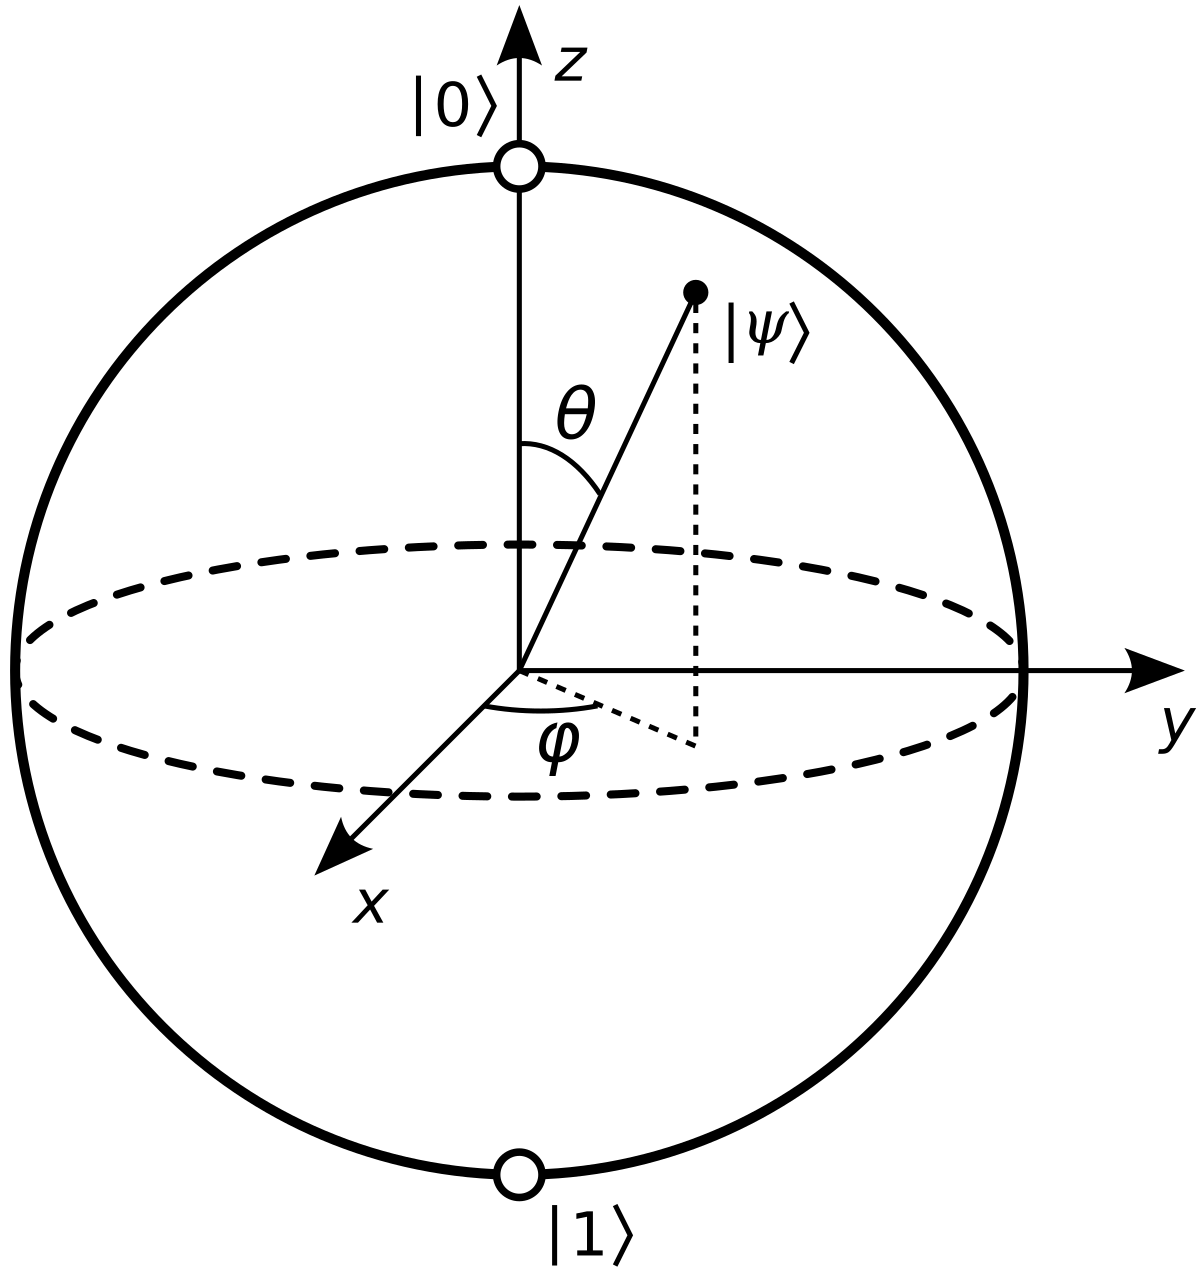
\includegraphics[width=0.4\textwidth]{Bloch_sphere.png}
    \caption{The Bloch sphere representation of a qubit, from reference [26].}
    \label{fig:bloch}
\end{figure}


\noindent The Bloch sphere is useful intuitively, as unitary transformations can be viewed as rotations about the axes. It's also useful for understanding the effects of measurement and decoherence, which collapse or shrink the qubit state towards the classical states. This section is supported by the definitions in source [9].



\subsection{Multi-Qubit State}

For  multi-qubit systems, the combined state space is the tensor product of the individual Hilbert spaces, as in section 2.6. For two qubits the joint system lives in a four-dimensional Hilbert space $\mathbb{C}^2 \otimes \mathbb{C}^2 = \mathbb{C}^4$, with the basis states:
\[
\{ |00\rangle, |01\rangle, |10\rangle, |11\rangle \}.
\]
\noindent Following from this since qubits live in a two-dimensional space we can infer that an $n$-qubit system spans a $2^n$-dimensional space as mentioned in [29]. This exponential growth in dimensions is why quantum computers can process large amounts of data in parallel as stated in [9].

\noindent The state of a multi-qubit system can be written as a superposition of these basis states. For example,  A two-qubit state is:
\[
|\psi\rangle = \alpha_{00}|00\rangle + \alpha_{01}|01\rangle + \alpha_{10}|10\rangle + \alpha_{11}|11\rangle,
\]
where $\alpha_{ij} \in \mathbb{C}$ and $\sum |\alpha_{ij}|^2 = 1$\\

\noindent In section 2.6.1 and 2.6.2 the examples we looked at for separable and entangled states were both two-qubit systems, The entangled state being the bell state [24], [25], and as we will see this is a crucial resource to quantum computers. Also we will see that quantum gates can actually generate entanglement of qubits.

\noindent It is also important to recall from Sections 2.3.4 and 2.6.3 that qubits and multi-qubit systems can be described using density matrices, both reduced and full [24],[25]. When only part of a system can be measured, reduced density matrices allow us to predict measurement outcomes, compute expectation values, and observe the local effects of quantum gates. They also help model the loss of quantum information due to entanglement with the environment, which leads to decoherence and errors in quantum systems [34].




\section{Quantum Circuits \& Gates}

\noindent Quantum circuits are made from applying multiple quantum gates to one or more qubits. As stated in Chapter 2, these unitary operators (logic gates) satisfy \( U^\dagger U = I \), this is why they're reversible and preserve probabilities until measurement.

\noindent In this section, we will define common quantum gates, for single qubits and multiple qubits, and show how they form quantum circuits. These concepts will be used later to construct algorithms and demonstrate quantum speedups.


\subsection{Single-Qubit Gates}

Single-qubit gates are applied to individual qubits to manipulate their state. As these gates are unitary operators they correspond to, $2$x$2$ complex matrices. Common single-qubit gates include:

\noindent\textbf{Pauli Gates}\\ 
\noindent The three Pauli gates, $X$, $Y$, and $Z$, are essentially 180° rotations around the $x$, $y$, and $z$ axes of the Bloch sphere [37]. They are represented by the corresponding $2$x$2$ matrices introduced in section 2.2.1.

\noindent The $X$ gate is like a classical NOT gate it flips $|0\rangle \leftrightarrow |1\rangle$, so for superpositions it switches the probability amplitudes. The $Z$ gate doesn't affect $|0\rangle$ but flips the sign of $|1\rangle$, changing the relative phase. The $Y$ gate is similar but with a complex phase. This can be backed up by [38]. \\

\noindent\textbf{The Hadamard Gate}\\
\noindent The Hadamard gate transforms the computational basis states into equal superpositions, $|+\rangle$, $|-\rangle$ and is represented by the matrix $H$:
\[
H = \frac{1}{\sqrt{2}} \begin{pmatrix} 1 & 1 \\ 1 & -1 \end{pmatrix},
\]
\[
H|0\rangle = \frac{1}{\sqrt{2}}
\begin{pmatrix}
1 & 1 \\
1 & -1
\end{pmatrix}
\begin{pmatrix}
1 \\
0
\end{pmatrix}
= \frac{1}{\sqrt{2}}
\begin{pmatrix}
1 \\
1
\end{pmatrix}
= \frac{1}{\sqrt{2}}(|0\rangle + |1\rangle)=|+\rangle,
\]

\[
H|1\rangle = \frac{1}{\sqrt{2}}
\begin{pmatrix}
1 & 1 \\
1 & -1
\end{pmatrix}
\begin{pmatrix}
0 \\
1
\end{pmatrix}
= \frac{1}{\sqrt{2}}
\begin{pmatrix}
1 \\
-1
\end{pmatrix}
= \frac{1}{\sqrt{2}}(|0\rangle - |1\rangle)=|-\rangle
\]\\
\noindent This operation moves qubits from the poles to the equator of the Bloch sphere [37], this gate creates superposition states allowing for interference.

\noindent $H$ is unitary and hermitian, so we have $H=H^\dagger$ and $H^\dagger H=HH^\dagger = I$, hence $HH=I$, this indicates that after applying the Hadamard gate, if it's applied again then the qubit states returns to the poles/are unaffected.
\\

\noindent\textbf{Phase Gates}\\
\noindent Phase gates are gates that apply phase shifts of the form $e^{\pi\varphi}$ (where $\varphi \in [0 ,2\pi]$), to just the $|1\rangle$ component of a qubit. Two common ones are the $S$ and $T$ gates:
\[
S = \begin{pmatrix} 1 & 0 \\ 0 & i \end{pmatrix}, \quad
T = \begin{pmatrix} 1 & 0 \\ 0 & e^{i\pi/4} \end{pmatrix}
\]
These gates don't affect $|0\rangle$. They rotate the qubit around the Bloch sphere’s z-axis. We can see from this that the Pauli $Z$ gate is also a phase gate. [38].



\subsection{Multi-Qubit Gates}

Multi-qubit gates are also unitary operators but they act on multiple qubits, they are used to entangle qubits. Arguably the most fundamental is the CNOT (controlled-not) gate.

\noindent The CNOT gate acts on two qubits, one is called the control the other is called the target. If the control qubits state is $|0\rangle$ then the target qubits state doesn't change. If the control qubits state is $|1\rangle$ then the target qubits state is flipped. The CNOT gate is represented by a $4$x$4$ matrix: 

\[
\text{CNOT} =
\begin{pmatrix}
1 & 0 & 0 & 0 \\
0 & 1 & 0 & 0 \\
0 & 0 & 0 & 1 \\
0 & 0 & 1 & 0
\end{pmatrix}.
\]\\
\noindent In the basis $\{|00\rangle, |01\rangle, |10\rangle, |11\rangle\}$. This gate can entangle two qubits when paired with the Hadamard gate as we will see in a later example. The CNOT gate is also well explained in [9].

\noindent Other notable multi-qubit gates include the CZ (controlled-Z) gate and the CCNOT (Toffoli) gate [29]. The CZ gate works similarly to the CNOT, it also uses a control and target qubit, if the control qubit $|0\rangle$ then the target qubits state doesn't change. But if the control qubits state is $|1\rangle$ then instead a phase shift is applied to the target qubit. The Toffoli gate is a three qubit gate that flips a target qubit if the two other qubits are both in the state $|1\rangle$ [29].


\subsection{Circuit Diagrams}

Quantum circuits are commonly represented using circuit diagrams, where the time progresses from left to right. This visual representation gives us a clear, organised way to describe sequences of gates operating on various qubits.

\noindent\textbf{Syntax} \\
\noindent Each line represents a qubit. A box with a gate name inside represents a single-qubit gate. Whereas, multi-qubit gates are shown by solid dots on the control qubits and $\oplus$ on the target qubit, connected by a vertical line. Measurement is denoted by a meter symbol or a half stadium shape with an $M$ inside. Finally, classical bits are represented by double horizontal lines. [39].

\subsubsection{Example Circuit}  
This example will show applying the Hadamard gate followed by the
CNOT gate creates an entanglement. Specifically, how the two-qubit state $|00\rangle$ becomes a Bell state:


\noindent First we apply a Hadamard gate to one of the qubits, lets say qubit one:

\[
|00\rangle \xrightarrow{H \otimes I} \frac{1}{\sqrt{2}} (|0\rangle + |1\rangle) \otimes |0\rangle
= \frac{1}{\sqrt{2}} (|00\rangle + |10\rangle),
\]

\noindent If the control is in a superposition when applying a CNOT you use the rule of the CNOT on each component of the superposition state, therefore applying the CNOT gate with qubit one as the control and two as the target:

\[
\frac{1}{\sqrt{2}} (|00\rangle + |10\rangle)\xrightarrow{\text{CNOT}} \frac{1}{\sqrt{2}} (|00\rangle + |11\rangle),
\]

\noindent This gives the entangled Bell state $|\Phi^+\rangle$ which we have seen from the examples in sections 2.6.2 and 2.6.3 is in fact entangled. We can visualise this process using this quantum circuit diagram: 
\[
\Qcircuit @C=1em @R=.7em {
& \lstick{|0\rangle} & \gate{H} & \ctrl{1} & \qw \\
& \lstick{|0\rangle} & \qw & \targ & \qw
}
\]

\noindent\textbf{Measurement in Circuits} \\
\noindent Normally at the end of a quantum circuit the qubits are measured, collapsing the states to $|0\rangle$ or $|1\rangle$ with probabilities as seen in 3.3.1. For the example bell state above, measurement over the basis $\{|00\rangle, |01\rangle, |10\rangle, |11\rangle\}$ will give the resultant states $|00\rangle$ and $|11\rangle$ with equal probabilities.

\section{Quantum Computing Algorithms}


Quantum algorithms use concepts from quantum theory to their advantage to make certain computations more efficiently than classical algorithms. Generally they start by initialising the qubits states, then a sequence of gates are applied to the qubits, and finally they are measured extracting classical results. This, as shown above, is implemented using a quantum circuits. The efficiency quantum algorithms have at specific computations is more accurately from: Superposition, namely its' ability to represent many possible inputs at once, enabling the evaluation of many inputs simultaneously. Interference, enabling quantum algorithms to steer towards the correct solution via constructive and destructive interference of probability amplitudes. Finally, entanglement, the strong correlation between qubits allows them to work together in a sense, improving the processing speed of information.


\subsection{Example Algorithm: Grover's Algorithm}
\noindent Grover’s algorithm [28] is a quantum search algorithm that's faster than typical classical search algorithms for unsorted lists. The algorithm goes as follows: 

\noindent Consider a function \( f: \{0, 1\}^n \rightarrow \{0, 1\} \) in which there is an input \( x_0 \) where \( f(x_0) = 1 \), and \( f(x) = 0 \) for all other \( x \)'s. We want to find \( x_0 \). Lets say the space the inputs live in has $ N \equiv 2^n$ items, this means $log_2(N) \equiv n$ qubits would allow the algorithm work on all possible inputs simultaneously in a superposition. This leads to the fact that while a standard classical search has an \( O(N) \) time efficiency, Grover’s algorithms is \( O(\sqrt{N}) \).\\

\noindent\textbf{Step 1 Initializing}\\
\noindent First we start all qubits in the zero state ( \( |0\rangle^{\otimes n} \)) and apply the Hadamard gate to each of them to make the system into a uniform superposition of all the possible inputs:

\[
|\psi\rangle = \frac{1}{\sqrt{N}} \sum_{x=0}^{N-1} |x\rangle.
\]\\

\noindent\textbf{Step 2: Oracle Marking}\\
\noindent An oracle \( O_f \) is then applied to the superposition state $|\psi\rangle$. The oracle is a sequence of quantum gates that flips the phase of the goal state (making its probability amplitude negative) while leaving all other states unchanged, essentially marking it. It can be written as:

\[
O_f |x\rangle = (-1)^{f(x)} |x\rangle.
\]

\noindent When applying this to $|\psi\rangle$, to mark \( |x_0\rangle \) we get:

\[
O_f |\psi\rangle = \frac{1}{\sqrt{N}} \sum_{x=0}^{N-1} (-1)^{f(x)} |x\rangle,
\]\\
\noindent\textbf{Step 3 Amplitude Amplification}\\
\noindent Next, a diffusion operator is applied to amplify the amplitude of the marked state by increasing its own amplitude and decreasing the amplitudes of all the others. This operator takes the average of the amplitudes and flips each amplitude around the average by the difference between the two. This operator is defined as:

\[
D = 2|\psi\rangle\langle\psi| - I.
\]

\noindent\textbf{Step 4 Iteration and Measurement}\\
\noindent The oracle and amplification steps by themselves don't seem very impactful but when they are iterated many times they increase the probability of the target outcome being measured immensely. A good example of how these steps work in tandem can be found in source [29] example 6.4.1. The optimal number of iterations before measurement to maximise probability of success with minimal number of iterations is $\frac{\pi}{4} \sqrt{N}
$ this is shown in source [30]. \\

\noindent\textbf{Note }Grover's algorithm is a solid example of an algorithm that uses the concepts of quantum theory namely, superposition and interference of probability amplitudes to its advantage. While, it produces a significant speedup there are other quantum algorithms like shor's that produce an exponential speedup.




\subsection{Programming on Quantum Computers}

Quantum algorithms can be made and executed using real or simulated quantum hardware. One of the most common tools for quantum programming is Qiskit, a framework modelled on python, made by IBM. Qiskit enables the construction of quantum circuits and consequently algorithms using python code, simulating their behaviour, or running them on IBM’s public quantum processors. The standard procedure of quantum programming is:
\begin{enumerate}
    \item Importing/loading Qiskit modules like \texttt{QuantumCircuit}, \texttt{Aer}, and \texttt{execute}.
    \item Initializing a quantum register (a system of qubits).
    \item Creating a sequence of gates.
    \item Adding measurement operations for extracting the resultant states of the qubits and storing them as classical information.
    \item Finally, Using a simulator or real quantum computer via the cloud to execute the program and collect the measurement results.
\end{enumerate}

\noindent One of my goals for this research project was to learn the basics of Qiskit and provide an example program that I've written. I have written a simple piece of code that demonstrates how Qiskit works and some of the key principles/fundamentals we've discussed, this can be seen in appendix B.






%--------------------------------------------------------------------
%	CONCLUSION
%--------------------------------------------------------------------

\newpage


\chapter{Conclusion}

This report formulated the key concepts of quantum theory bridging the gap from the abstract mathematical representation to in practice quantum computation. We started by introducing the linear algebra framework used to describe quantum states, superposition, entanglement and more. We then contextualised these fundamentals in the realm of quantum computing, describing qubits and how they are manipulated by quantum operators. Finally, we looked at the practical implementation via an example algorithm (Grover's search algorithm) and the use of Qiskit programming. 

\noindent One key idea we can take away is that quantum computing is superior under specific circumstances compared to its classical counterpart. The use of superposition, interference and entanglement enables significant speedups, but currently only for the certain algorithms/problems that take advantage of them.

\noindent Another point worth noting is, while there are accessible tools for working with quantum computers such as IBM's Qiskit and cloud quantum processors, there still doesn't exist a general purpose quantum computer that can be used for a range of applications. This is because of the numerous challenges that still exist in quantum computing. Currently, the cost to build and maintain quantum computers is very high, this is due to the massively difficult engineering needed for such a project. This stems from the environment quantum computers require to function as intended, which includes extreme conditions, such as near absolute zero temperatures and minimal disturbances, because of the fragility of qubits. This comes from trying to account for the issue of noise and decoherence (when the quantum system interacts with the environment losing its ability to utilise quantum phenomena). Decoherence is also a bottleneck for scalability as adding more qubits to the system magnifies the noise and decoherence causing the addition of each extra qubit to be exponentially complex. One technique that aims to counter decoherence is error correction, in source [1] it's emphasised that this is critical for increasing scalability. Today's machines still operate with a considerable level of noise, but during the time of writing this report there has been progress on this with the new topological architecture qubit made by Microsoft[31], that is stated to have massively larger scalability and fault tolerance potential.

\noindent There are many types of physical architectures of qubits as all that is essentially necessary is any two-level quantum system, common architectures include: ion traps, where the two-level system is the two energy levels of the ion, another is linear optical photons, where the two-level system is the two distinct optical
paths the photon can travel down. There are many more that we can't look into during this report, for more extensive detail you can refer to source [32].

\noindent Quantum computers are projected to make an impact in many fields ranging from materials science to cryptography. One example of a near future application is quantum key distribution (QKD) this a line of communication, provably safe from eavesdropping. There are already experiments being done using satellites to demonstrate QKD and quantum teleportation [33]. Another field with massive potential is quantum simulation, the capability that quantum computers possess in simulating quantum systems including modelling complex molecules is something classical computers can't match, [34] for further reading. There is also the question of what does AI look like when synergised with quantum computers? This is an area with massive potential for breakthroughs in drug discoveries and other areas, you can see this is interlinked with quantum simulation quite heavily source [35] goes into more detail on the topic.

\noindent We can conclude by saying quantum computing is a field that unifies mathematics, physics and computer science. It's technology that's directly developed from the linear algebra mathematics of quantum theory. While still not a fully realised field, there are rapid advancements happening and massive potential applications. It is a testament to how mathematics can drive technological revolutions.




%--------------------------------------------------------------------
%	FINAL REFLECTIONS
%--------------------------------------------------------------------

\newpage

\addcontentsline{toc}{chapter}{Final Reflections}

\chapter*{Final Reflections}

My initial aim for this project was to explore quantum computing from its mathematical foundations, through to its logic, and into its applications, with a focus on quantum cryptography. This was a wide scope that I planned. It included concepts from superposition and entanglement to Shor's algorithm and even philosophical implications. This is evidenced by the evolution of my title from “Introduction to Quantum Computing” in the project plan, to “Evolution of Quantum Computing: Foundations, Practical Impacts and Challenges” in my draft, and then “The Mathematics of Quantum Theory \& Computing” in my final report. You can see as I got deeper into my research I realised, to go into sufficient depth on each point I would have to sacrifice elements. While editing I decided to prioritise a thorough mathematical foundation and the fundamental logic of quantum computing. I would then mention topics that I had cut in the conclusion, adding suggestions for further reading. However, I was unable to include all topics, one example is Shor's algorithm, while having impactful applications, it wasn't fit for the report due to it's complexity because of its reliance on quantum Fourier transforms. I cut philosophical implications as I was unable to find notable sources. 

\noindent A challenge I faced early in the process was the amount of mathematics in quantum theory I was unfamiliar with. Concepts like Tensor products, Hilbert spaces, Quantum Operators and partial traces were initially overwhelming. Early on, while I still wasn't comfortable with these concepts, I visited sources multiple times to fully understand. This led to a change in my approach, I started rephrasing definitions and arguments and trying out examples where I was less confident. This slowed my pace but helped me gain a deeper understanding of the content, through correcting mistakes or positive reinforcement.

\noindent A big moment came when I started researching entanglement. I already had an informal idea of entanglement, and in conjunction with my understanding of the mathematical representation of superposition, I thought if two quantum states formed a superposition and were expressible by a third, they were entangled. I realised this mistake as I did further research into entangled states. I found how critical tensor products are and I'd been unaware of the key idea of entanglement, separable vs non-separable states. This mistake led me down the path of loss of information and finding reduced density matrices. It also brought more new mathematics like partial traces. This challenge helped me gain a much deeper understanding of entanglement, a principle that would be fundamental going forward.

\noindent The research process deviated considerably from the project plan. Initially, I had planned on covering error correction and quantum cryptography, but to achieve this with sufficient detail I would have needed to go into group representation theory and quantum information theory. Instead, I expanded my knowledge of linear algebra and operator theory. Another significant pivot was when I decided to hone in on Grovers algorithm as I could explain it more succinctly and also use it to create an example Qiskit program simulating its operation.

\noindent I used feedback from my supervisor to improve the structure and accuracy of my report. For example, he informed me of the controversy surrounding Google's claims of quantum supremacy and IBM's criticism. The advice to keep my research relevant to what I will be covering later on, helped me minimise time wasted researching areas that didn't have relevance. The focus on Grover's algorithm over Shor's algorithm also came through discussion of realistic aims for the project.

\noindent This project has helped develop my mathematical research skills. I learnt that making mistakes is an important step for gaining a deeper understanding. My latex and time management skills improved by deconstructing tasks into small achievable goals and setting soft deadlines on myself.

\noindent If I did the project again, I would want to define the fundamentals of quantum computing and the mathematical foundations simultaneously, so that I'm able to go into detail on quantum teleportation with a Qiskit implementation and subsequently quantum encryption methods (quantum key encryption). After completing this project I feel I'm now better equipped for future research into areas I'm interested in like quantum machine learning and simulation.


%--------------------------------------------------------------------
%	REFERENCES
%--------------------------------------------------------------------

\newpage

\addcontentsline{toc}{chapter}{References}

\chapter*{References}

[1] Preskill, J., \textit{Quantum Computing and the Entanglement Frontier}, arXiv:1203.5813, 2012. Available at: https://arxiv.org/pdf/1203.5813\\

\noindent[2] Arute, F., et al., \textit{Quantum Supremacy using a Programmable Superconducting Processor}, Nature, vol. 574, pp. 505–510, 2019. Available at: https://www.nature.com/articles/s41586-019-1666-5\\

\noindent[3] Dirac, P. A. M., \textit{The Principles of Quantum Mechanics}, 4th ed., Oxford University Press, 1958.\\

\noindent[4] Pednault, E., Maslov, D., Gunnels, J., Gambetta, J., \textit{IBM Quantum Computing Blog | On “quantum supremacy”}, Available at: https://www.ibm.com/quantum/blog/on-quantum-supremacy, Visited March 08, 2025.\\

\noindent [5] Busch, P., Heinonen, T., \& Lahti, P., \textit{Heisenberg's Uncertainty Principle}, arXiv:quant-ph/0609185v3, 2007. Available at: https://arxiv.org/abs/quant-ph/0609185 \\

\noindent[6] Artin, M., \textit{Algebra}, Pearson, 2010.\\

\noindent[7] Hoffman, K., \& Kunze, R., \textit{Linear Algebra}, Prentice-Hall, 1971.\\

\noindent[8] Axler, S., \textit{Linear Algebra Done Right}, Springer, 1997.\\

\noindent[9] Nielsen, M. A., \& Chuang, I. L., \textit{Quantum Computation and Quantum Information}, Cambridge University Press, 2010.\\

\noindent[10] Meyer, C. D., \textit{Matrix Analysis and Applied Linear Algebra}, SIAM, 2000.\\

\noindent[11] Sakurai, J. J., \& Napolitano, J., \textit{Modern Quantum Mechanics}, 3rd ed., Cambridge University Press, 2020.\\

\noindent[12] Arias-Castro, E., \textit{Principles of Statistical Analysis}, v1.0, University of California, San Diego, 2021.\\

\noindent[13] Hall, B. C., \textit{Quantum Theory for Mathematicians}, Springer, 2013.\\

\noindent[14] Rynne, B., and Youngson, M., \textit{Linear Functional Analysis}, Springer, 2008.\\

\noindent[15] Easttom, C., \textit{Quantum Computing Fundamentals}, Addison-Wesley, 2021. Available at: https://ptgmedia.pearsoncmg.com/images/9780136793816/samplepages/9780136793816\_Sample.pdf\\

\noindent[16] Griffiths, D. J., \textit{Introduction to Quantum Mechanics}, 2nd ed., Pearson Prentice Hall, 2005.\\

\noindent[17] Koprinkov, I. G., \textit{Spatial, Temporal and Coherent Superposition of Quantum States, a Reinterpretation of the Superposition Principle}, Journal of Modern Physics, Vol. 15, No. 2, pp. 183–197, 2024. Available at: https://www.scirp.org/journal/paperinformation.aspx?paperid=137875\\

\noindent[18] Marinescu, D. C., \& Marinescu, G. M., \textit{Classical and Quantum Information}, Academic Press, 2011.\\

\noindent[19] Greenberger, D., Hentschel, K., \& Weinert, F. (Eds.), \textit{Compendium of Quantum Physics: Concepts, Experiments, History and Philosophy}, Springer, 2009.\\

\noindent[20] Tokmakoff, A., \textit{Time-Dependent Quantum Mechanics and Spectroscopy}, University of Chicago, Lecture Notes.\\

\noindent[21] Feynman, R. P., Leighton, R. B., \& Sands, M., \textit{The Feynman Lectures on Physics, Vol. 3}, Addison-Wesley, 1965.\\

\noindent[22] Kalami Heris, M., \textit{Unveiling the Inner Product: The Key to Similarity in Math, Machine Learning, and Beyond}, Available at: https://kalami.medium.com/unveiling -the-inner-product-the-key-to-similarity-in-math-machine-learning-and-beyond-290b43cf34fd, Visited March 30, 2025.\\

\noindent[23] Peeters, K., \textit{Commutators and the Uncertainty Principle}, University of Durham, Available at: https://www.maths.dur.ac.uk/users/kasper.peeters/mathphys/uncertainty.html, Visited March 30, 2025.\\

\noindent[24] Maziero, J., \textit{Computing Partial Traces and Reduced Density Matrices}, arXiv:1601.07458, 2016. Available at: https://arxiv.org/pdf/1601.07458\\

\noindent[25] LaRose, R., \textit{Quantum States and Partial Trace}, QuIC Seminar 6, Michigan State University, 2018. Available at: https://www.ryanlarose.com/uploads/1/1/5/8/115879647/quic06-states-trace.pdf\\

\noindent[26] Wikipedia- Smite-Meister , \textit{Bloch sphere}, Wikipedia, The Free Encyclopedia. Available at: https://en.wikipedia.org/wiki/Bloch\_sphere, Visited April 2, 2025.\\

\noindent[27] Ladyman, J., Presnell, S., Short, A. J., \& Groisman, B., \textit{The connection between logical and thermodynamic irreversibility}, Studies in History and Philosophy of Modern Physics, Vol. 38, Issue 1, 2007. Available at: https://www.sciencedirect.com/science/article/pii/S1355219806000682\\

\noindent[28] Grover, L. K., \textit{A fast quantum mechanical algorithm for database search}, arXiv:quant-ph/9605043, 1996. Available at: https://arxiv.org/abs/quant-ph/9605043\\

\noindent[29] Yanofsky, N. S., \& Mannucci, M. A., \textit{Quantum Computing for Computer Scientists}, Cambridge University Press, 2008. Available at: https://quantumatlas.ir/wp-content/uploads/2025/01/Quantum-Computing-for-Computer
\noindent-Scientists.pdf\\

\noindent[30] IBM Quantum Learning, Fundamentals of Quantum Algorithms \textit{Grover's Algorithm}, Available at: https://learning.quantum.ibm.com/course/fundamentals-of-quantum-algorithms
\noindent/grovers-algorithm, Visited April 5, 2025.\\

\noindent[31] Youvan, D., \textit{Microsoft's Majorana 1: A Paradigm Shift Toward Scalable and Fault-Tolerant Quantum Computing}, 2025. Available at: https://doi.org/10.13140/RG.2.2.11176.89607\\

\noindent[32] Microsoft Quantum, \textit{Types of Qubits}, Microsoft Quantum Documentation. Available at: https://quantum.microsoft.com/en-us/insights/education/concepts/types-of-qubits, Visited April 6, 2025.\\

\noindent[33] Bedington, R., Arrazola, J. M., \& Ling, A., \textit{Progress in Satellite Quantum Key Distribution}, npj Quantum Information, vol. 3, article 30, 2017. Available at: https://doi.org/10.1038/s41534-017-0031-5\\

\noindent[34] Georgescu, I. M., Ashhab, S., \& Nori, F., \textit{Quantum Simulation}, Reviews of Modern Physics, vol. 86, no. 1, pp. 153–185, 2014. Available at: https://doi.org/10.1103/RevModPhys.86.153\\

\noindent[35] Alexeev, Y., Farag, M. H., Patti, T. L., Wolf, M. E., Ares, N., Aspuru-Guzik, A., Benjamin, S. C., Cai, Z., Chandani, Z., Fedele, F., Harrigan, N., Kim, J.-S., Kyoseva, E., Lietz, J. G., Lubowe, T., McCaskey, A., Melko, R. G., Nakaji, K., Peruzzo, A., Stanwyck, S., Tubman, N. M., Wang, H., \& Costa, T., \textit{Artificial Intelligence for Quantum Computing}, arXiv:2411.09131 [quant-ph], 2024. Available at: https://arxiv.org/abs/2411.09131\\


\noindent[36] Brandão, F. G. S. L., Christandl, M., Harrow, A. W., \& Walter, M., \textit{The Mathematics of Entanglement}, arXiv:1604.01790, 2016. Available at: https://arxiv.org/pdf/1604.01790\\

\noindent[37] Elbaset, M. A., Deraz, S. A., Soliman, M. A., \& Moussa, K. H., \textit{A 32-bit Quantum Encryption Algorithm Using Dynamic Pauli Gates}, 2023. Available at: https://www.researchgate.net/publication/372648350\_A\_32-bit\_Quantum\_Encryption\_
\noindent Algorithm\_Using\_Dynamic\_Pauli\_Gates\\

\noindent[38] Lambropoulos, P., \& Petrosyan, D., \textit{Fundamentals of Quantum Optics and Quantum Information}, Springer, 2007. Available at: https://www.researchgate.net/publication/253619080\_Fundamentals\_of\_Quantum\_Optics\_
\noindent and\_Quantum\_Information\\

\noindent[39] IBM Quantum Learning, \textit{Quantum Circuits}, Available at: https://learning.quantum.ibm.com/course/basics-of-quantum-information/quantum-circuits, Visited April 4, 2025.\\




%-------------------------------------------------------------------
%	APPENDICES
%-------------------------------------------------------------------

\newpage
\appendix

\chapter{Extra Definitions}
\label{appendix:A}

\subsubsection{Fields}
\noindent This definition uses the following reference for inspiration [6].

\noindent A \textbf{field} \( \mathbb{F} \) is a mathematical structure consisting of a set of elements equipped with two binary operations: \textbf{addition} and \textbf{multiplication}, which satisfy the following properties:

\begin{enumerate}
    \item \textbf{Closure}: If \( a, b \in \mathbb{F} \), then \( a + b \in \mathbb{F} \) and \( a \cdot b \in \mathbb{F} \).
    \item \textbf{Commutativity}: \( a + b = b + a \) and \( a \cdot b = b \cdot a \).
    \item \textbf{Associativity}: \( (a + b) + c = a + (b + c) \) and \( (a \cdot b) \cdot c = a \cdot (b \cdot c) \).
    \item \textbf{Distributive Law}: \( a \cdot (b + c) = a \cdot b + a \cdot c \).
    \item \textbf{Additive identity}: There exists an element \( 0 \in \mathbb{F} \) such that for all \( a \in \mathbb{F} \), we have \( a + 0 = a \).
    \item \textbf{Multiplicative identity}: There exists an element \( 1 \in \mathbb{F} \), with \( 1 \neq 0 \), such that for all \( a \in \mathbb{F} \), we have \( a \cdot 1 = a \).
    \item \textbf{Additive inverse}: For each \( a \in \mathbb{F} \), there exists \( -a \in \mathbb{F} \) such that \( a + (-a) = 0 \).
    \item \textbf{Multiplicative inverse}: For each \( a \neq 0 \), there exists \( a^{-1} \in \mathbb{F} \) such that \( a \cdot a^{-1} = 1 \).
\end{enumerate}

\noindent \textbf{Note:} you could also condense this to three axioms; \( \mathbb{F} \) forming two abelian groups, one with the binary operation + and the other with the binary operation \(\cdot\) and the distributive law must hold.
\noindent \textbf{Example Fields} include \( \mathbb{R} \), \( \mathbb{C} \), and \( \mathbb{Z}/p\mathbb{Z} \) (finite fields)\\


\subsubsection{Vector Spaces}

A \textbf{vector space} is made up of four components:
\begin{enumerate}
    \item \textbf{A field} \( \mathbb{F} \): This is the scalars of the vector space. If it is useful to specify the field then the vector space is referred to as a vector space over the field \( \mathbb{F} \)
    \item \textbf{A set of vectors \( V \)}: As long as there is no ambiguity then we just refer to the whole vector space as \( V \)
    \item \textbf{Vector addition}: \( +: V \times V \to V \), satisfying commutativity, associativity, and the existence of an additive identity vector \( \mathbf{0} \) and additive inverses \( -\mathbf{v} \).
    \item \textbf{Scalar multiplication}: \( \cdot: \mathbb{F} \times V \to V \), satisfying distributivity (for \( a (\mathbf{u} + \mathbf{v}) = a\mathbf{u} + a\mathbf{v} \) and \( (a + b)\mathbf{v} = a\mathbf{v} + b\mathbf{v} \)), associativity, and the existence of a multiplicative identity \( 1 \in \mathbb{F} \).
\end{enumerate}

\noindent These operations satisfy closure: \( \mathbf{u} + \mathbf{v} \in V \) and \( a\mathbf{v} \in V \) for all \( \mathbf{u}, \mathbf{v} \in V \) and \( a \in \mathbb{F} \).
This definition was constructed with the help of reference [7].


\subsubsection{Expected Values}
\noindent \textbf{Expected values} are like the average result of all the possible outcomes. They are weighted based on the probability of each outcome occurring. The expected value can be calculated for discrete variables by:
\begin{equation}
\mathbb{E}[X] = \sum_i x_i \cdot P(x_i)
\end{equation}
Where $X$ is a random variable that takes the values \(x_i\) with probabilities \( P(x_i) \).

\subsubsection{Probability Distributions}
A \textbf{Probability distribution} is simply a function P that maps all possible outcomes to a value for probability. satisfying the following:
\begin{enumerate}
    \item All probabilities must be between 0 and 1, \(0\leq P(x_i) \leq 1\)
    \item All probabilities must sum to 1, \(\sum_i P(x_i) = 1\)
\end{enumerate}


\chapter{Qiskit Code}
\label{appendix:B}

\begin{lstlisting}[language=Python, caption={Forming the Bell state $|\Phi^+\rangle = \frac{1}{\sqrt{2}} (|00\rangle + |11\rangle)$}]
import qiskit
from qiskit import QuantumCircuit
from qiskit_aer import AerSimulator
from qiskit.visualization import plot_histogram
import matplotlib.pyplot as plt 
from IPython.display import display, clear_output
clear_output(wait=True)
%matplotlib inline
#Creates circuit with all qubits initialized to the state |0>
bell_circuit = QuantumCircuit(2, 2)

# Create superposition and entanglement
bell_circuit.h(0)  # Apply Hadamard to qubit 0
bell_circuit.cx(0, 1)  # Entangle with qubit 1 by using CNOT

# Add measurement
bell_circuit.measure([0, 1], [0, 1])
print("Circuit diagram")
display(bell_circuit.draw('mpl', style='bw'))

# Simulate the measurement
result = simulator.run(bell_circuit, shots=1000).result()
counts = result.get_counts()

# Display results
print("\nMeasurement results")
display(plot_histogram(counts, title="Measurement results", bar_labels=True))
plt.close('all')
\end{lstlisting}


\subsubsection{Output:}
\begin{figure}[H]
    \centering
    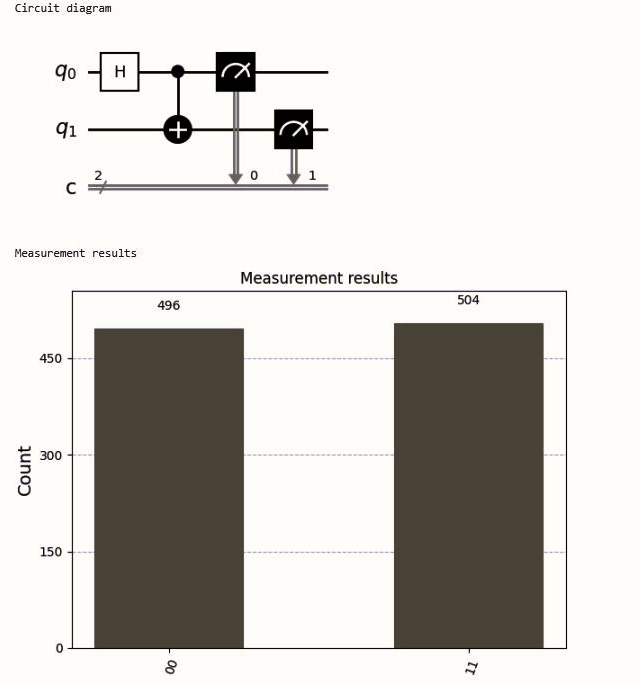
\includegraphics[width=1.1\textwidth]{Bell-state-output.png}
    \label{fig:output1}
\end{figure}
\newpage

\begin{lstlisting}[language=Python, caption={3 Qubit Grover search for the state $|101\rangle$}]
from qiskit import transpile
import numpy as np

target = '101'
iterations = 2  #The optimal number of iterations is pi/4 * sqrt(2^3) which is 
                 #approximately 2

#Creates circuit with all qubits initialized to the state |0>
grover = QuantumCircuit(3, 3)

#Puts all qubits into equal superpositions
grover.h([0, 1, 2])

#Iterative steps
for _ in range(iterations):
    #The oracle operator for |101>
    grover.x(1)  #We need to flip this qubit to convert |101> to |111> as 
                  #the CCZ gate phase just flips |111>
    grover.h(2)
    grover.ccx(0, 1, 2)  #phase flip
    grover.h(2)
    grover.x(1)
    
    #The diffusion operator
    grover.h([0, 1, 2])
    grover.x([0, 1, 2])
    grover.h(2)
    grover.ccx(0, 1, 2)
    grover.h(2)
    grover.x([0, 1, 2])
    grover.h([0, 1, 2])

#Measurement
grover.measure([0, 1, 2], [0, 1, 2])
print("\nCircuit Diagram")
grover.draw('mpl', style='bw', fold=12, cregbundle=False)

#Simulate results
result = AerSimulator().run(grover, shots=1000).result()
counts = result.get_counts()


#Output simulated measurement results
all_states = [format(i, '03b') for i in range(2**3)]
complete_counts = {state: counts.get(state, 0) for state in all_states}
plot_histogram(complete_counts,
               title=f"Measurement results with target |{target}\rangle",
               bar_labels=True)
plt.tight_layout()
plt.show()

print(f"\nProbability of success is {counts.get(target, 0)/1000:.1%}")

\end{lstlisting}

\subsubsection{Output:}
\begin{figure}[H]
    \centering
    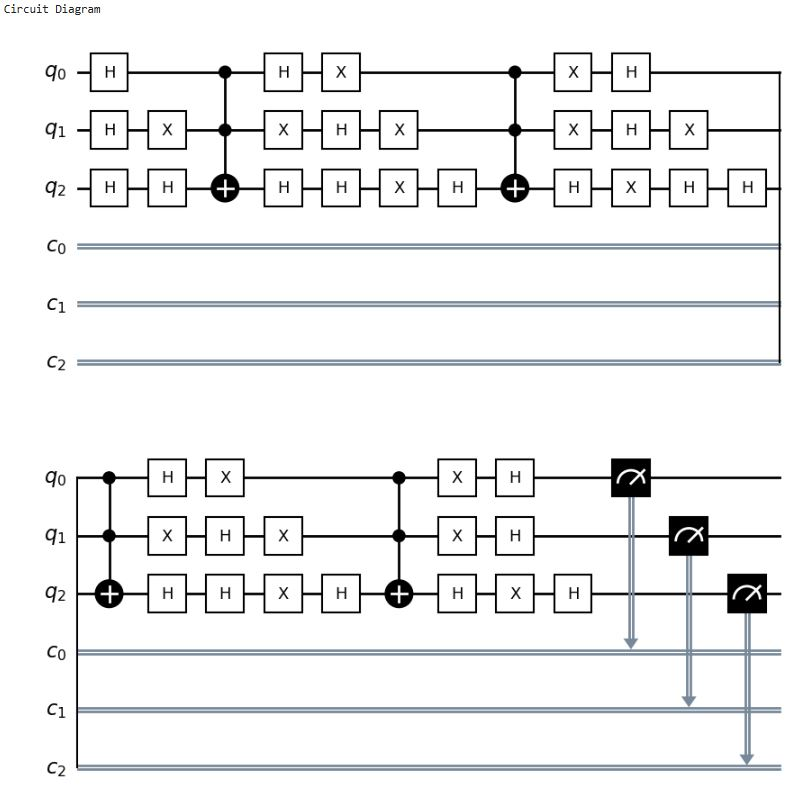
\includegraphics[width=\textwidth]{Grovers-circuit-diagram.png}
    \label{fig:output2}
\end{figure}

\begin{figure}[H]
    \centering
    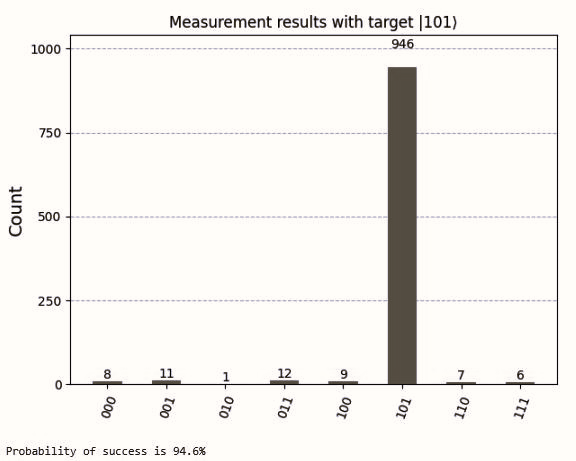
\includegraphics[width=1.0\textwidth]{Grovers-measurement-results.png}
    \label{fig:output3}
\end{figure}

%-------------------------------------------------------------------

\end{document}  
